% MedVision manuscript V2, targeted to the Journal of Biomedical Informatics.
% The original MedVision_Q1_Master.tex and its component files are intentionally
% not imported or modified. This file is a self-contained journal-specific manuscript
% that reuses only the verified bibliography and figure assets.

\documentclass[a4paper,fleqn]{cas-sc}

\usepackage{amsmath,amssymb}
\usepackage{booktabs}
\usepackage{float}
\usepackage{placeins}
\usepackage{graphicx}
\usepackage{multirow}
\usepackage[numbers,sort&compress]{natbib}
\usepackage{xcolor}
\usepackage{hyperref}
\hypersetup{hypertexnames=false,hidelinks}
\Urlmuskip=0mu plus 2mu\relax

\graphicspath{{figures/}}

\setlength{\floatsep}{7pt plus 2pt minus 2pt}
\setlength{\textfloatsep}{8pt plus 2pt minus 2pt}
\setlength{\intextsep}{8pt plus 2pt minus 2pt}
\interfootnotelinepenalty=10000

% Keep the manuscript visually clean while retaining page numbers.
\ExplSyntaxOn
\cs_set:Npn \__first_footerline: {}
\cs_set:Npn \__first_head: {}
\cs_set:Npn \__cas_head: {}
\ExplSyntaxOff
\RenewDocumentCommand \printorcid { } { }
\pagestyle{cas}

\begin{document}

\title[mode=title]{Quantifying Modality Inertia in Medical Vision-Language Models: Image Contribution Metric, Gate Stagnation, and the Failure of Debiasing Under Label Circularity}

\author{Nafis Al Rahman}
\author{Tanvir Mahmud}

\begin{abstract}
\textbf{Objective:} Medical vision-language models may obtain high scores from
radiology reports without using corresponding images. This risk is acute when
evaluation labels and model text inputs share report provenance. We evaluated
whether text-debiasing increased incremental image information in a
MIMIC-CXR-derived classification task and assessed an Image Contribution Metric
(ICM) as a modality-use audit.

\textbf{Methods:} We analysed 2,953 frontal studies assigned at patient level
to training (2,049), validation (449), and test (455) sets. Five fusion
conditions were evaluated across eight seeds: baseline gated fusion, a learned
text-prior product-of-experts variant, a noise-sensitivity (anti-consistency)
condition, an exploratory
grounding-aware variant, and an adaptive-gate variant. The primary intervention
replaced the radiograph with a constant gray image while preserving the report.
ICM measured the relative Macro-F1 difference between the full model and this
Gray-Square control. Seed-level inference included signed-rank tests, two
one-sided tests within an operational equivalence interval of -0.01 to 0.01,
bootstrap intervals, calibration analysis, and retained checkpoint-gate
inspection.

\textbf{Results:} Baseline Macro-F1 was $0.9397\pm0.0061$; the retained
Gray-Square control achieved 0.9381. Baseline ICM was $0.0016\pm0.0065$
(95\% bootstrap confidence interval $[-0.0026,0.0061]$). The signed-rank test
was non-significant ($p=0.4219$), whereas the equivalence test supported an ICM
inside the operational interval ($p=0.0040$). No intervention produced a
robust ICM increase. The text-prior variant increased expected calibration
error from 0.0237 to 0.0621 and Brier score from 0.0522 to 0.0685. Retained
baseline gates remained near their class-specific initial values, with an
overall mean of 0.49975.

\textbf{Conclusions:} In this report-linked benchmark, near-ceiling
classification was compatible with negligible incremental image contribution.
ICM and gate inspection expose a construct-validity problem that aggregate
performance alone cannot detect. The result is specific to this cohort and
archived implementation; independent labels, matched controls, validation of
preprocessing and objectives, provenance locking, and external validation are
required before clinical or general claims.
\end{abstract}

\begin{keywords}
medical vision-language model \sep biomedical informatics \sep label circularity
\sep shortcut learning \sep modality inertia \sep Image Contribution Metric
\sep equivalence testing \sep MIMIC-CXR
\end{keywords}

\begingroup
\sloppy
\maketitle
\endgroup

\section*{Statement of significance}
Biomedical informatics studies increasingly combine images and text, but a
multimodal score does not reveal which input supplied the decisive information.
This study addresses a specific threat to validity: CheXpert targets and the
model's report input share linguistic provenance. We combine a report-preserving
image intervention, a seed-level ICM, calibration analysis, and retained-gate
inspection to distinguish multimodal performance from incremental visual
evidence. The audit shows how apparently strong performance can persist after
removing image information and provides a reproducible reporting pattern for
benchmark designers, clinical-AI evaluators, and researchers assessing modality
reliance. ICM is proposed as a diagnostic measure, not a standalone certificate
of grounding.

\section{Introduction}\label{sec:introduction}

Medical vision-language models (VLMs) offer a natural way to combine the
complementary information in radiographs and radiology reports. Large paired
resources such as MIMIC-CXR support representation learning, classification,
report generation, and clinical question answering at a scale that would be
difficult to obtain through manual annotation alone \cite{johnson2019mimiccxr}.
Contrastive and local-alignment approaches, including ConVIRT, GLoRIA, and
BioViL, have shown that report semantics can improve biomedical image
representations \cite{zhang2022convirt,huang2021gloria,boecking2022textsemantics}.
The clinical interpretation of a downstream score nevertheless depends on a
more basic question: did the declared image input materially affect the model's
decision?

High accuracy cannot answer that question. Deep networks can learn predictive
features that are stable within a benchmark but unrelated to the intended
mechanism \cite{geirhos2020shortcut}. In radiology, acquisition hardware,
population composition, annotation practice, and clinical context can each
create shortcuts \cite{gichoya2023shortcuts}. Multimodal systems introduce an
additional route: a strong language pathway may dominate a weaker visual
pathway. Correct answers can then coexist with flawed image rationales, stable
outputs can survive removal of the image, and a plausible heatmap can be
mistaken for evidence of causal grounding
\cite{jin2024hiddenflaws,lotfinia2026needimage,sadanandan2026consistentdangerous}.
Recent chest-radiography studies further show that performance claims can change
when the amount or relevance of clinical context changes
\cite{wang2026clinicalcontext}. These observations make modality contribution
an empirical estimand rather than an architectural assumption.

Label provenance makes the problem sharper in MIMIC-CXR-derived tasks. CheXpert
maps radiology-report language to uncertainty-aware pathology labels
\cite{irvin2019chexpert}. If the same report, or its \texttt{findings} field,
is supplied to the predictor, the text input and target share an information
source. A model can therefore be rewarded for recognizing language that helped
produce the label. Report-conditioned prediction may still serve a useful
informatics purpose, but it is not equivalent to independent image-based
recognition. Natural-language labelers also have their own error modes and
potential subgroup effects, which can propagate into any downstream evaluation
\cite{sabottke2024targetselection,santomartino2024nlplabeling}.

Standard debiasing methods do not automatically resolve this circularity.
Visual-question-answering methods reduce language or answer priors by
penalizing an easy unimodal pathway or combining it with a multimodal expert
\cite{agrawal2018dontassume,clark2019easyway,cadene2019rubi}. Their logic assumes
that the bias pathway is a nuisance proxy rather than a near-direct encoding of
the benchmark target. When report text is also the label source, suppressing the
text pathway may discard information rewarded by the endpoint without creating
an independent visual signal. A lower score then shows that text mattered, not
that image use improved. Prototype and counterfactual methods can produce more
interpretable predictions, but explanation quality remains distinct from
behaviour under a controlled input intervention \cite{chiang2026cxrnexus}.

Three evidentiary gaps remain. First, few studies replace the radiograph while
holding report, label, architecture, and test cohort fixed. Second, a balanced
fusion gate or attention coefficient is often treated as attribution even
though it may remain near initialization \cite{arevalo2017gmu}. Third,
non-significance is sometimes described as proof of no modality contribution,
although failure to reject zero and evidence of equivalence are different
statistical conclusions \cite{lakens2017equivalence}. Together, these gaps can
make a nominally multimodal model appear visually grounded when the evaluation
has not tested that claim.

We address these gaps in a controlled audit of a three-class
MIMIC-CXR-derived task comprising Normal, Pneumonia, and Pneumothorax. We
compare the full model with a report-preserving Gray-Square intervention,
text-only and image-only controls, and four fusion or text-debiasing variants
alongside the baseline gated model. The primary diagnostic is the Image
Contribution Metric (ICM), the relative Macro-F1 difference between a full VLM
and its Gray-Square reference. We pair ICM with an operational equivalence test,
calibration metrics, class-specific performance, gate inspection, and
qualitative Grad-CAM \cite{selvaraju2017gradcam}. The study asks whether
removing image information changes predictive performance, whether the tested
interventions increase incremental image contribution, and whether retained
gates provide evidence of learned visual reliance. It is a benchmark audit,
not a new clinical predictor and not a claim that radiographs are generally
unnecessary.

\section{Related work}\label{sec:related-work}

\textbf{Medical image-text learning and report-derived targets.}
Paired image-report learning has improved transfer and label efficiency by
using free text as a rich source of supervision. ConVIRT uses contrastive
learning across paired views; GLoRIA models global and local correspondences;
and BioViL emphasizes biomedical text semantics
\cite{zhang2022convirt,huang2021gloria,boecking2022textsemantics}. Clinical BERT
representations similarly improve the handling of biomedical terminology,
negation, and context \cite{alsentzer2019clinicalbert,devlin2019bert}. These
advances establish the utility of text but do not by themselves identify the
incremental contribution of the image in a downstream task. That question is
especially consequential when labels are automatically extracted from the same
reports used during prediction.

\textbf{Shortcut learning and unimodal bias.}
Shortcut learning describes reliance on an easy predictive signal that performs
well in-distribution but does not match the intended construct
\cite{geirhos2020shortcut}. Language priors are a long-standing example in
visual question answering. VQA-CP, ensemble-based debiasing, product-of-experts
objectives, and RUBi attempt to reduce this dependence by exposing or
down-weighting the language-only expert
\cite{agrawal2018dontassume,clark2019easyway,cadene2019rubi}. In a medical
benchmark with report-derived targets, however, the language pathway is not
merely correlated with the outcome: it participates in the outcome-generation
process. The present study evaluates whether methods borrowed from the former
setting retain their intended meaning in the latter.

\textbf{Auditing modality reliance.}
Recent evaluations separate output correctness from evidence dependence.
Multimodal answers can have unreliable visual rationales, and predictions can
remain consistent even when the image is uninformative
\cite{jin2024hiddenflaws,sadanandan2026consistentdangerous}. Controlled image
removal, cross-patient replacement, and text-only comparisons have shown that
several chest-radiography VLMs retain substantial performance without the image
\cite{lotfinia2026needimage}. Clinical context can also alter apparent model
quality \cite{wang2026clinicalcontext}. These studies motivate behavioural
interventions but generally do not combine a per-model relative contribution
metric, equivalence testing, seed-level calibration, and gate inspection in one
audit.

\textbf{Gates and explanation limits.}
Gated multimodal units provide a compact mechanism for combining modality
representations \cite{arevalo2017gmu}. A gate value is nevertheless a model
parameter, not a causal estimate. A non-zero gate may be unidentifiable when
both pathways encode redundant signals, or it may stay near initialization if
the objective supplies little incentive to move it. The same caution applies to
attention and saliency: a visually plausible map does not show that removal of
the highlighted evidence changed the output. Reasoning-oriented radiography
models and prototype methods may improve transparency, but their explanations
remain complementary to input interventions
\cite{myronenko2025reasoningcxr,chiang2026cxrnexus}. We therefore position ICM
as an intervention-based diagnostic and treat gates and Grad-CAM only as
supporting observations.

\section{Methods}\label{sec:methods}

\subsection{Study design, data source, and cohort}\label{sec:study-design}

We performed a retrospective computational audit. The estimand was incremental
image contribution when the report remained available. The principal
intervention replaced each radiograph by a constant gray tensor while retaining
the report, target, fusion path, and evaluation cohort. Full multimodal outputs
were compared with this report-preserving control and with descriptive
text-only and image-only controls. Figure~\ref{fig:design}(a--c) presents the
proposed visual organization of the image pathway, report pathway, and audit
workflow; the archived implementation is specified in
Section~\ref{sec:architecture}. Figure~\ref{fig:design}(d) records cohort
selection and the patient-level split.

\begin{figure}[pos=p]
\centering
% Panels (a)--(c) are already labelled within the supplied artwork.
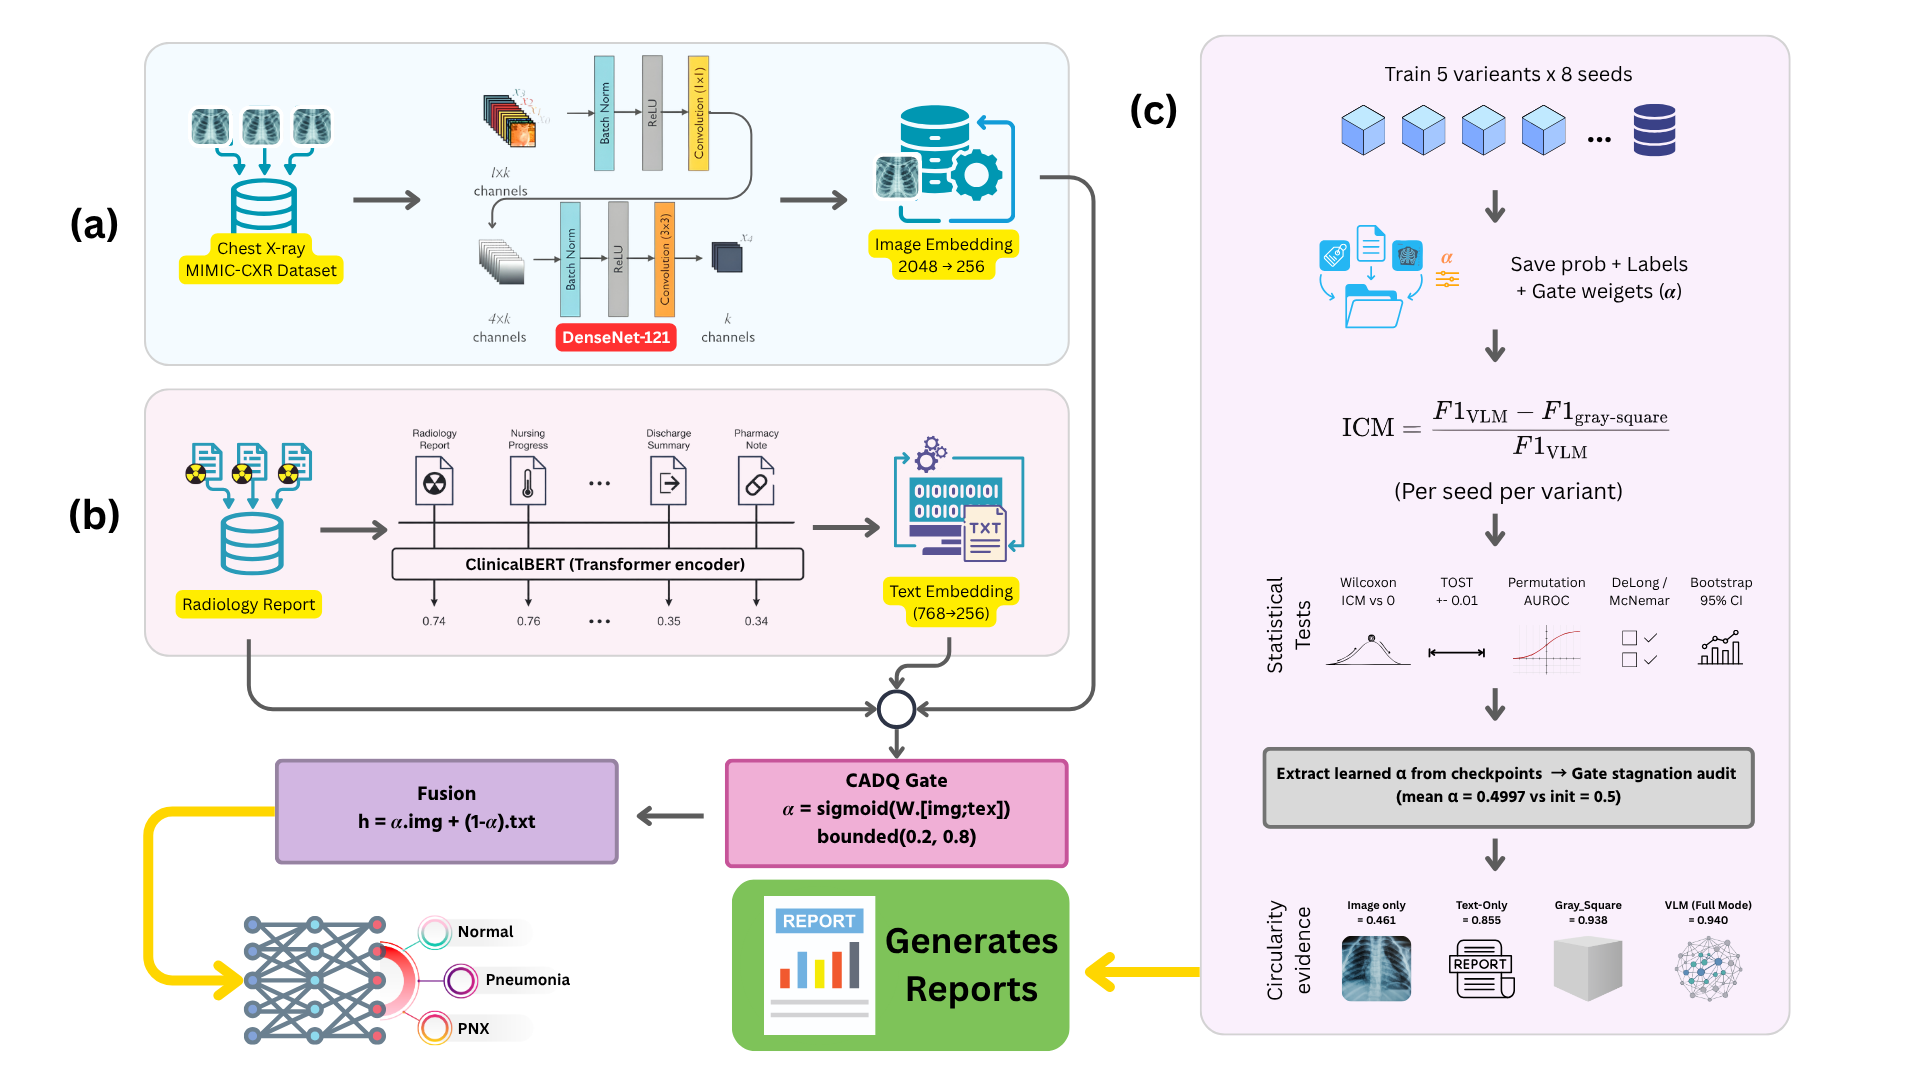
\includegraphics[width=\linewidth]{methodology_diagram_v2_abc.png}\par\medskip
\textbf{(d)}\par\smallskip
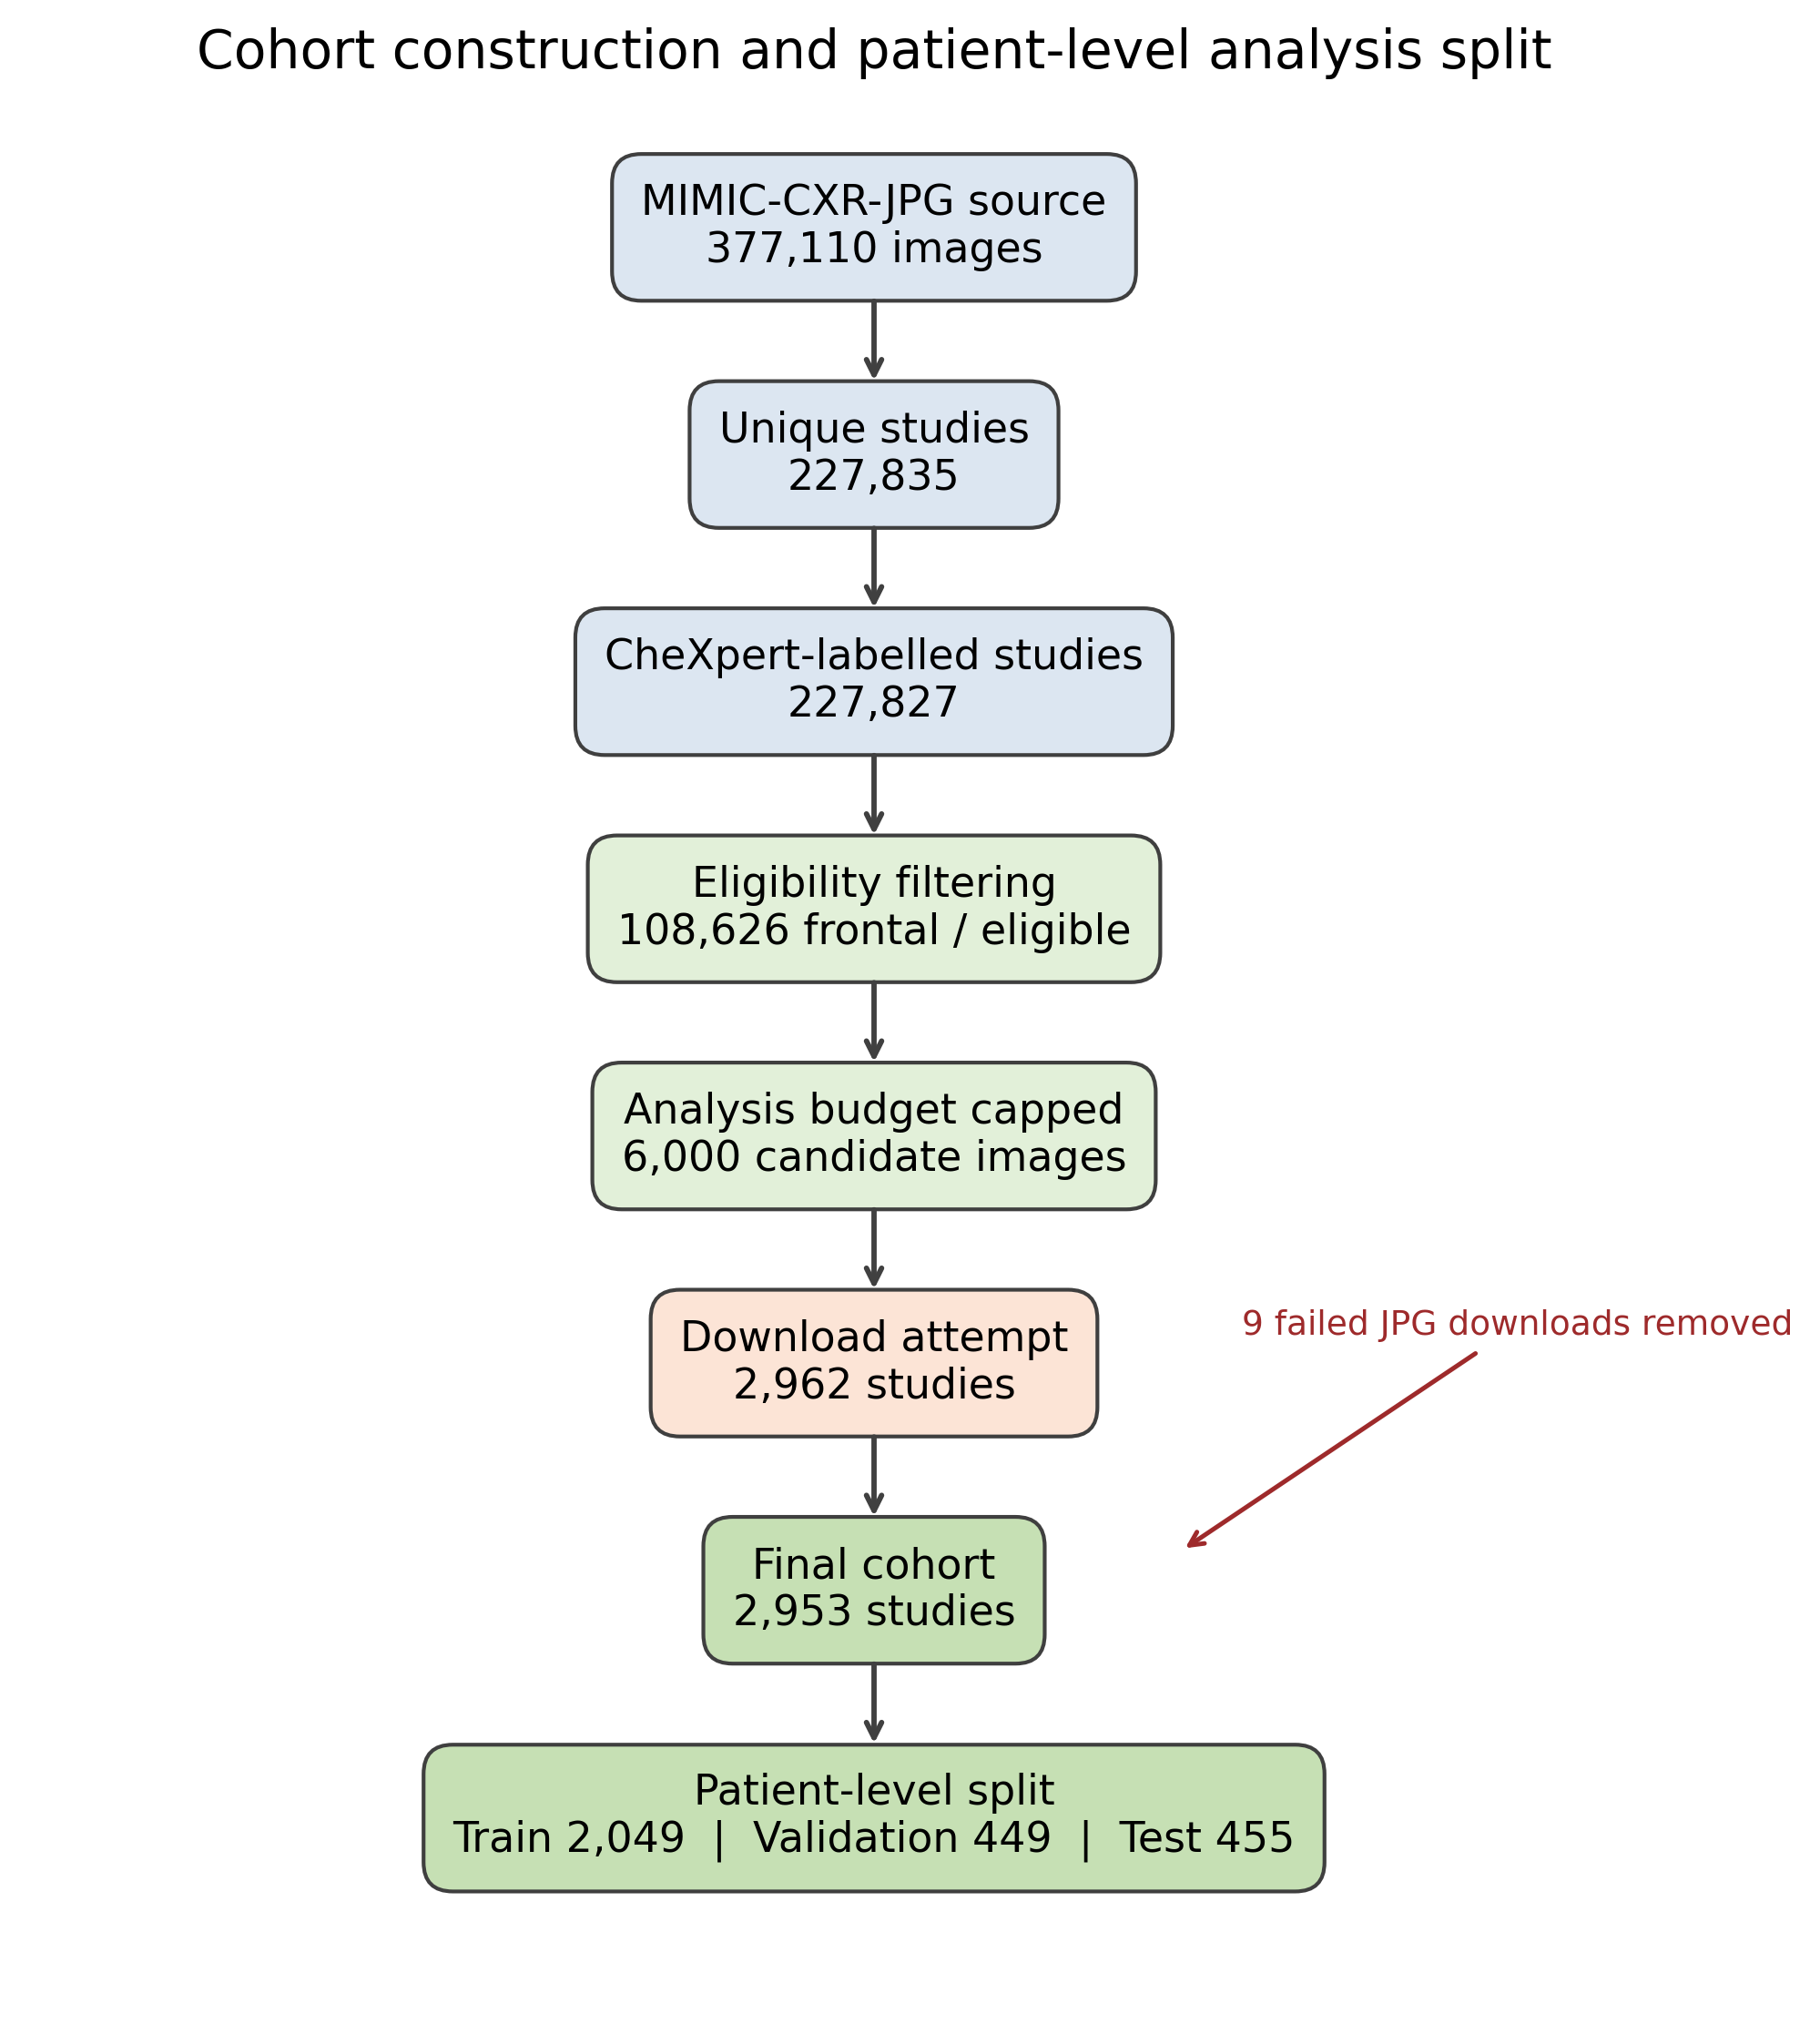
\includegraphics[height=0.35\textheight,keepaspectratio]{cohort_flow.png}
\caption{Study design and proposed schematic. (a) Image pathway.
(b) Report pathway and fusion. (c) Five-condition, eight-seed audit workflow,
ICM, retained-gate inspection, and controls. Panels (a--c) reproduce a working
schematic pending implementation alignment: the archived model used
512-dimensional projections, findings-only Bio\_ClinicalBERT input, single-key
attention, and a static per-class baseline logit gate, not the displayed
input-dependent feature gate. It predicted classes, not reports. The displayed
permutation analysis is not part of the reported inference; DeLong and McNemar
used retained seed-42 outputs, and each control had one retained run. These
panel details must not be read as additional experiments.
(d) Retained cohort-construction flow: nine unavailable JPG files were removed
before the final 2,953-study cohort was partitioned at patient level.}
\label{fig:design}
\end{figure}

MIMIC-CXR JPG images and reports were accessed through official PhysioNet
credentialing under the applicable Data Use Agreement
\cite{johnson2019mimiccxr}. The source flow comprised 377,110 images in 227,835
studies; 227,827 studies had CheXpert labels and 108,626 met the frontal-view
eligibility criteria. An analysis cap selected up to 2,500 Normal, 2,500
Pneumonia, and 1,000 Pneumothorax candidates. Of 2,962 attempted downloads,
nine JPG files were unavailable, leaving 2,953 usable studies. The inherited
patient-level GroupShuffleSplit assigned 2,049 studies to training, 449 to
validation, and 455 to test, with no subject overlap. The test set contained
240 Normal, 168 Pneumonia, and 47 Pneumothorax studies.

CheXpert generated the targets from report language using the project's
uncertain-to-negative mapping \cite{irvin2019chexpert}; the model received the
same report's \texttt{findings} field. The experiment consequently audits
label-report circularity rather than an independent radiograph-only diagnostic
task. The replication unit for seed-level inference was a trained model at a
fixed seed. Baseline CADQ, LearnedMixinFusion (LMH), noise-sensitivity
(anti-consistency), exploratory GACR-B, and Adaptive-CADQ each had eight
retained seeds: 42, 123, 456, 789, 1010, 1111, 1212, and 1313. The eight-seed
plan covered baseline, LMH, and noise-sensitivity (anti-consistency);
Adaptive-CADQ was extended from three to eight seeds after the initial run, and
exploratory GACR-B was added post hoc. The latter two analyses are
therefore exploratory.

\subsection{Preprocessing and architecture}\label{sec:architecture}

The \texttt{findings} field was tokenized with
\texttt{emilyalsentzer/Bio\_ClinicalBERT}, truncated or padded to 256 tokens,
and randomly replaced by an empty string in 10\% of training examples. Test and
validation text was not masked. Images were converted to one channel, resized
to $256\times256$, randomly cropped to $224\times224$ during training, and
mapped from $[0,255]$ to $[-1,1]$. Training augmentation used horizontal
flipping, rotation up to $10^{\circ}$, translation, and brightness/contrast
jitter; the minority-class transform increased the rotation, translation,
scale, shear, jitter, and blur ranges. Validation and test preprocessing was
deterministic. The archived $[-1,1]$ mapping may not match the native
TorchXRayVision normalization expected by the selected weights; this is an
implementation limitation that should be addressed in a confirmatory analysis
\cite{cohen2022torchxrayvision}.

The image branch used a TorchXRayVision DenseNet-121 with
\texttt{densenet121-res224-mimic\_ch} weights
\cite{huang2017densenet,cohen2022torchxrayvision}. All image-bearing fusion
conditions shared the same $[-1,1]$ intensity mapping. A deviation from the
native TorchXRayVision convention is therefore a shared preprocessing
limitation, but equal effects on absolute scores or unchanged within-study
contrasts cannot be assumed. ICM and condition contrasts characterize the
retained preprocessing setting.\footnote{\textbf{Internal wording proposal---
validation pending, not an observed finding:} ``All conditions shared a uniform
$[-1,1]$ intensity mapping; any deviation from the native TorchXRayVision
convention therefore acts as a shared preprocessing shift that affects absolute
scores equally across conditions and does not alter within-study contrasts.''
This proposal requires a matched normalization sensitivity analysis; a common
mapping alone does not establish equal effects.}
The encoder's convolutional stem and
first dense block were frozen, and its output was projected to 512 dimensions
through a linear layer, LayerNorm, Gaussian Error Linear Unit, and dropout
(0.25). The text branch used Bio\_ClinicalBERT with the first four transformer
layers frozen and an analogous 512-dimensional projection
\cite{devlin2019bert,alsentzer2019clinicalbert}. One projected image token was
used as the query and one projected text token as the key/value in an eight-head
attention block with residual LayerNorm. Because there is only one key, this
operation cannot express word-region alignment; we interpret it as feature
interaction, not causal attention.

Baseline CADQ combined image and text logits through a bounded learnable
per-class gate \cite{arevalo2017gmu}:
\begin{equation}
\alpha_c=0.20+0.60\operatorname{sigmoid}(u_c),\qquad
z_c=\alpha_c z^{\mathrm{img}}_c+(1-\alpha_c)z^{\mathrm{text}}_c.
\end{equation}
The initial logits $u=(-0.5,0,0.5)$ corresponded to image-gate values
$(0.426524,0.500000,0.573476)$ for Normal, Pneumonia, and Pneumothorax.

LMH added a five-fold out-of-fold term-frequency/inverse-document-frequency
logistic text prior (5,000 unigram/bigram features, stop-word removal, balanced
weights), temperature calibration, $\epsilon=0.1$ smoothing, an input-dependent
prior gate, and an entropy penalty of 0.05 annealed over three epochs. It was
warm-started from CADQ and followed the product-of-experts rationale used for
unimodal-bias reduction \cite{cadene2019rubi}. The noise-sensitivity
(anti-consistency) condition perturbed the
image with Gaussian noise ($\sigma=0.25$). Its archived objective added
$-D_{KL}(p_{clean}\|p_{noisy})$ to a minimized loss and therefore rewards
divergence; throughout this manuscript it is treated as a noise-sensitivity
(anti-consistency) condition, not a conventional consistency objective.
Adaptive-CADQ replaced the static per-class gate with a sample-dependent scalar
computed from image and text entropies by a $2\rightarrow16\rightarrow1$
multilayer perceptron. Exploratory GACR-B used an out-of-fold text baseline and
a cosine penalty of 0.3 on examples for which that baseline misclassified, following
the grounding-aware intervention of Sadanandan and Behzadan
\cite{sadanandan2026consistentdangerous}.

The image-only control used the image encoder with a 512-to-256 classifier; the
text-only control used frozen Bio\_ClinicalBERT with a 768-to-256 classifier.
The Gray-Square control replaced every image by a constant intensity-128 tensor
but preserved the report and multimodal architecture. Only one retained run was
available for each control. Gray-Square is therefore a report-preserving image
ablation, not an independently trained eight-seed text-only ensemble.

\subsection{Training and outcomes}\label{sec:training}

Models were trained for 10 epochs with AdamW and weight decay $10^{-4}$
\cite{loshchilov2019adamw}. Learning rates were $10^{-5}$ for the image and text
backbones, $10^{-4}$ for fusion and LMH heads, and $5\times10^{-5}$ for static
gates. OneCycleLR used 10\% warm-up \cite{smith2019superconvergence}. Physical
batch size was 8 with four gradient-accumulation steps (effective batch 32),
mixed precision, and gradient scaling. The objective combined focal
cross-entropy ($\gamma=1.5$), label smoothing (0.05), and effective-number class
weights ($\beta=0.99$) \cite{lin2017focalloss}. Class-aware sampling replicated
Pneumothorax examples up to fivefold and Pneumonia examples up to threefold.
The highest validation Macro-F1 checkpoint was restored for multimodal
conditions. The image-only control was retained as a descriptive capacity
probe; its archived pipeline did not guarantee restoration of the best
validation checkpoint. Inferential claims about modality reliance rest on the
report-preserving Gray-Square intervention, not the image-only result.\footnote{
\textbf{Internal wording proposal---validation pending, not the archived
checkpoint description:} ``The image-only control was retained as a descriptive
capacity probe without exhaustive checkpoint tuning; inferential claims about
modality reliance rest on the report-preserving Gray-Square intervention.''
Use this wording only after checkpoint restoration is verified and the
associated result is confirmed; tuning scope does not establish restoration
of the selected checkpoint.}

The primary diagnostic was
\begin{equation}
\mathrm{ICM}=\frac{F1_{VLM}-F1_{Gray}}{F1_{VLM}},
\end{equation}
where positive values indicate better Macro-F1 with the real radiograph. The
relative form was chosen to express the incremental change on the scale of the
full model. An ICM near zero indicates that replacing the image did not
materially change this endpoint; it does not prove that the image encoder is
universally uninformative. The analysis used an operational equivalence interval
of $[-0.01,0.01]$. This project-defined margin is neither a validated clinical
threshold nor a regulatory acceptance criterion.

Secondary outcomes were Macro-F1, accuracy, one-versus-rest Macro-AUROC,
per-class F1 and sensitivity, ten-bin expected calibration error (ECE),
multiclass Brier score, row-normalized confusion matrices, retained image-gate
values, and qualitative Grad-CAM. ECE and Brier were recomputed from retained
probability arrays when absent from the summary dictionary; missing values were
never replaced with zero. Gate values were taken from the per-seed checkpoint
export in \texttt{q1\_audit\_results.json}. The displayed gate figure uses all
eight exported values and their equation-derived initialization references,
rather than hard-coded aggregate values.

\subsection{Statistical analysis and reproducibility}\label{sec:statistics}

Seed-level differences used paired Wilcoxon signed-rank tests with Pratt zero
handling and paired $t$-tests. ICM summaries included the median, standard
deviation, Cohen's $d$, and percentile bootstrap 95\% confidence intervals from
2,000 resamples. Two one-sided tests (TOST) evaluated whether ICM lay within
$[-0.01,0.01]$ \cite{lakens2017equivalence}. Because the same 455 studies recur
at every seed, test subjects were not concatenated across seeds for
confirmatory inference.

DeLong tests compared correlated Pneumothorax receiver-operating-characteristic
curves within the retained seed-42 probability set \cite{delong1988roc}.
McNemar tests compared paired classification decisions on the same 455 seed-42
studies \cite{mcnemar1947correlated}. Benjamini-Hochberg correction controlled
the false-discovery rate within each test family
\cite{benjamini1995fdr}. A McNemar $p$-value of 1 denotes balanced discordance,
not identical predictions; the two off-diagonal counts are therefore reported
with the test result.

Python, NumPy, and PyTorch seeds were fixed and deterministic cuDNN settings
were enabled. Run metadata, validation histories, checkpoints, predictions,
probabilities, and configurations were retained. The fixed merge archive
resolved duplicate keys by the first-seen value, but the earlier workflow did
not preserve a deterministic source-priority rule and content-hash manifest.
Results are consequently tied to this archive snapshot. Reporting was audited
against CLAIM and TRIPOD+AI principles
\cite{mongan2024claim,collins2024tripodai}; checklist summaries and a provenance
manifest are included in the Supplementary material.

\section{Results}\label{sec:results}

\subsection{Analysis set, discrimination, and calibration}\label{sec:performance}

The fixed archive contained 40 condition-seed records: five conditions with
eight seeds each, evaluated on the same 455 held-out studies. Baseline CADQ
achieved Macro-F1 $0.9397\pm0.0061$, accuracy $0.9607\pm0.0032$, and
Macro-AUROC $0.9974\pm0.0004$ (Table~\ref{tab:performance}). LMH had the
highest mean Macro-F1 ($0.9435\pm0.0093$) but lower and more variable AUROC
($0.9849\pm0.0113$). The noise-sensitivity (anti-consistency) condition had
the lowest Macro-F1 ($0.9346\pm0.0075$). Exploratory GACR-B reached
$0.9417\pm0.0059$, and
Adaptive-CADQ remained close to baseline at $0.9388\pm0.0072$.

\begin{table}[pos=htbp]
\centering
\caption{Performance and calibration across eight seeds (mean $\pm$ standard
deviation). Exploratory GACR-B was added post hoc.}
\label{tab:performance}
\scriptsize
\setlength{\tabcolsep}{3.2pt}
\resizebox{\linewidth}{!}{%
\begin{tabular}{lccccc}
\toprule
Condition & Macro-F1 & Accuracy & Macro-AUROC & ECE & Brier \\
\midrule
Baseline CADQ & $0.9397\pm0.0061$ & $0.9607\pm0.0032$ & $0.9974\pm0.0004$ & $0.0237\pm0.0048$ & $0.0522\pm0.0040$ \\
LMH (PoE) & $0.9435\pm0.0093$ & $0.9596\pm0.0070$ & $0.9849\pm0.0113$ & $0.0621\pm0.0160$ & $0.0685\pm0.0213$ \\
Noise-sensitivity (anti-consistency) & $0.9346\pm0.0075$ & $0.9560\pm0.0039$ & $0.9960\pm0.0013$ & $0.0347\pm0.0137$ & $0.0655\pm0.0130$ \\
Exploratory GACR-B & $0.9417\pm0.0059$ & $0.9610\pm0.0042$ & $0.9972\pm0.0005$ & $0.0245\pm0.0023$ & $0.0540\pm0.0038$ \\
Adaptive-CADQ & $0.9388\pm0.0072$ & $0.9610\pm0.0044$ & $0.9972\pm0.0008$ & $0.0241\pm0.0070$ & $0.0527\pm0.0028$ \\
\bottomrule
\end{tabular}}
\end{table}

Baseline per-class F1 was $0.9755\pm0.0032$ for Normal,
$0.9624\pm0.0055$ for Pneumonia, and $0.8810\pm0.0174$ for
Pneumothorax. LMH increased Pneumothorax F1 to $0.9003\pm0.0191$ but
reduced Pneumonia F1 to $0.9575\pm0.0077$. The noise-sensitivity
(anti-consistency) condition had the
widest Pneumothorax variation ($0.8753\pm0.0237$). Adaptive-CADQ showed
the most stable Pneumonia F1 ($0.9616\pm0.0029$). The distributions and
the retained control contrast are shown in Figure~\ref{fig:performance-controls}.

\begin{figure}[pos=htbp]
\centering
\textbf{(a)}\par\smallskip
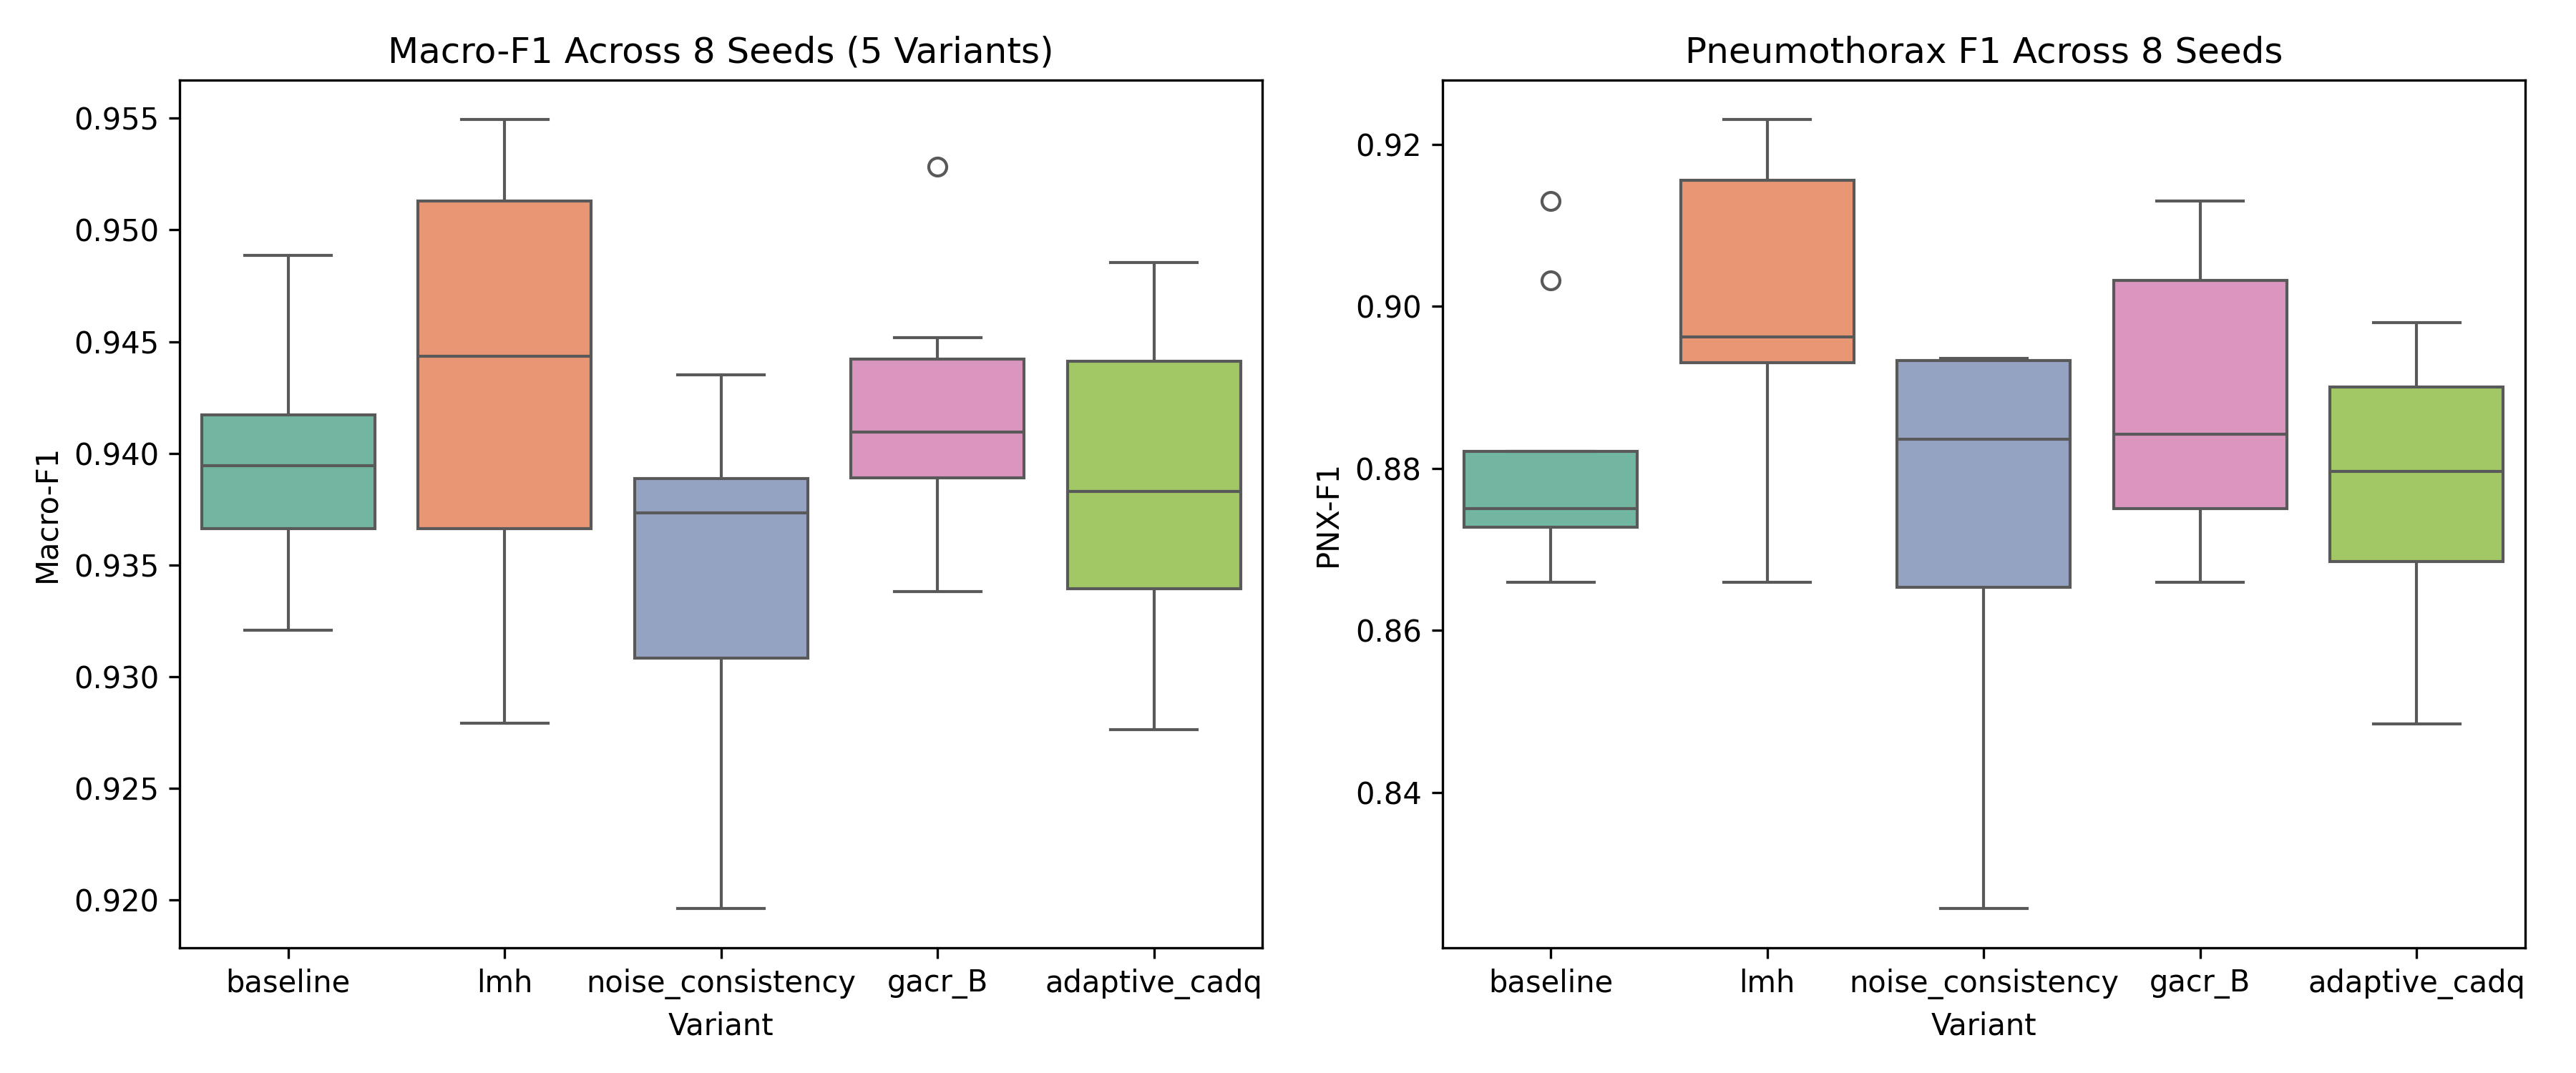
\includegraphics[width=0.88\linewidth]{f1_boxplots.png}\par\medskip
\textbf{(b)}\par\smallskip
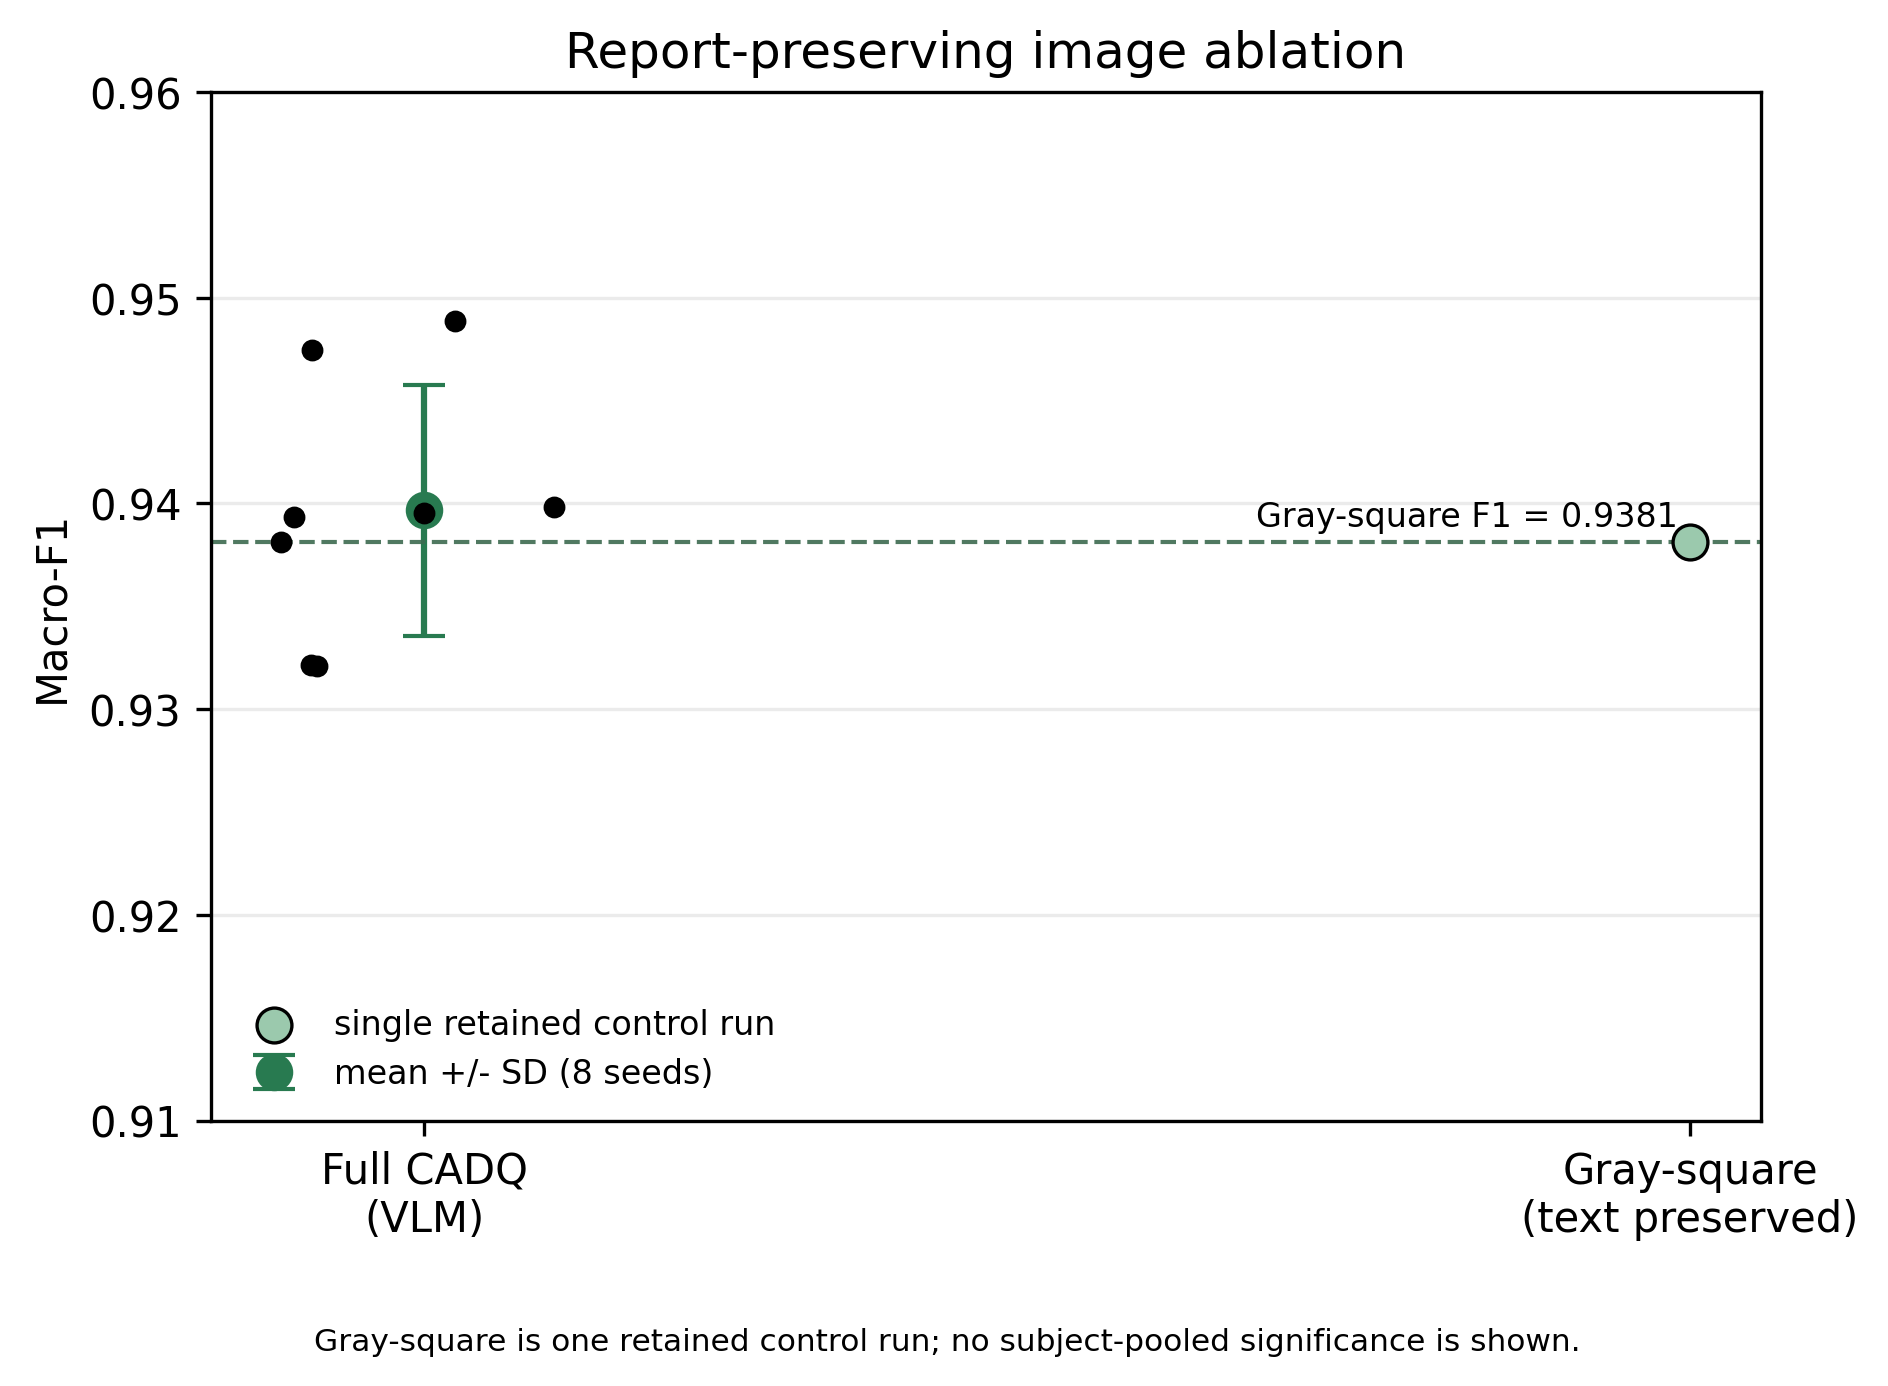
\includegraphics[width=0.61\linewidth]{circularity_contrast.png}
\caption{Predictive performance and controls. (a) Macro-F1 and
Pneumothorax-F1 distributions over eight seeds for the five fusion conditions.
(b) Retained single-run controls compared with the baseline VLM. Restoration of
the best validation checkpoint was not guaranteed for image-only evaluation,
and control values are descriptive rather
than modality rankings.}
\label{fig:performance-controls}
\end{figure}

No condition improved Macro-F1 over baseline after Benjamini-Hochberg
correction (Table~\ref{tab:pairwise}). The largest unadjusted Macro-F1 signal
was the exploratory GACR-B contrast ($\Delta=0.0020$, Wilcoxon $p=0.0547$;
adjusted $p=0.2188$). LMH and the noise-sensitivity (anti-consistency)
condition had lower seed-42
Pneumothorax AUROC than baseline; their significant DeLong results indicate
degradation, not improvement. Adaptive-CADQ showed no AUROC difference.

\begin{table}[pos=htbp]
\centering
\caption{Paired comparisons with baseline. Wilcoxon uses eight paired
seed-level Macro-F1 values. DeLong and McNemar use the retained seed-42
probability and prediction arrays for the same 455 studies. Values in
parentheses are Benjamini-Hochberg adjusted within each test family. McNemar
$n_{01}/n_{10}$ are the discordant counts; $p=1$ does not imply identical
predictions.}
\label{tab:pairwise}
\scriptsize
\resizebox{\linewidth}{!}{%
\begin{tabular}{lccc}
\toprule
Condition & Wilcoxon Macro-F1 $p$ (BH) & DeLong PNX-AUROC $p$ (BH) & McNemar $n_{01}/n_{10}$; $p$ (BH) \\
\midrule
LMH (PoE) & 0.2500 (0.3333) & $2.9\times10^{-6}$ ($1.2\times10^{-5}$) & 27/31; 0.6936 (1.0000) \\
Noise-sensitivity (anti-consistency) & 0.1953 (0.3333) & 0.0022 (0.0044) & 32/49; 0.0754 (0.3018) \\
Exploratory GACR-B & 0.0547 (0.2188) & 0.0315 (0.0420) & 9/8; 1.0000 (1.0000) \\
Adaptive-CADQ & 0.8438 (0.8438) & 0.7304 (0.7304) & 15/14; 1.0000 (1.0000) \\
\bottomrule
\end{tabular}}
\end{table}

The balanced discordance for exploratory GACR-B and Adaptive-CADQ is informative.
Exploratory GACR-B disagreed
with baseline on 17 studies (9 versus 8 across the two off-diagonal directions),
and Adaptive-CADQ on 29 (15 versus 14). McNemar $p=1.000$ indicates no evidence
of directional asymmetry in these paired errors; it does not indicate
byte-identical predictions. The confusion matrices and receiver-operating-
characteristic curves in Figure~\ref{fig:error-roc} are descriptive views of
the same repeated test cohort.

\begin{figure}[pos=htbp]
\centering
\textbf{(a)}\par\smallskip
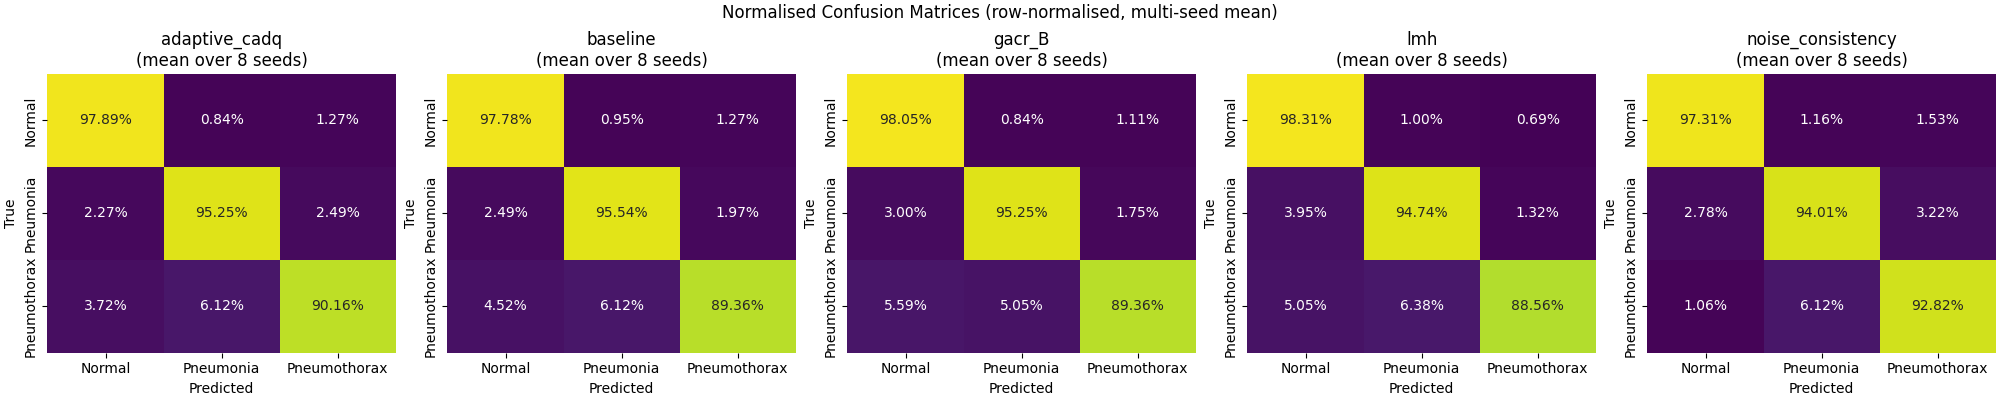
\includegraphics[width=0.92\linewidth]{confusion_matrices_normalised.png}\par\medskip
\textbf{(b)}\par\smallskip
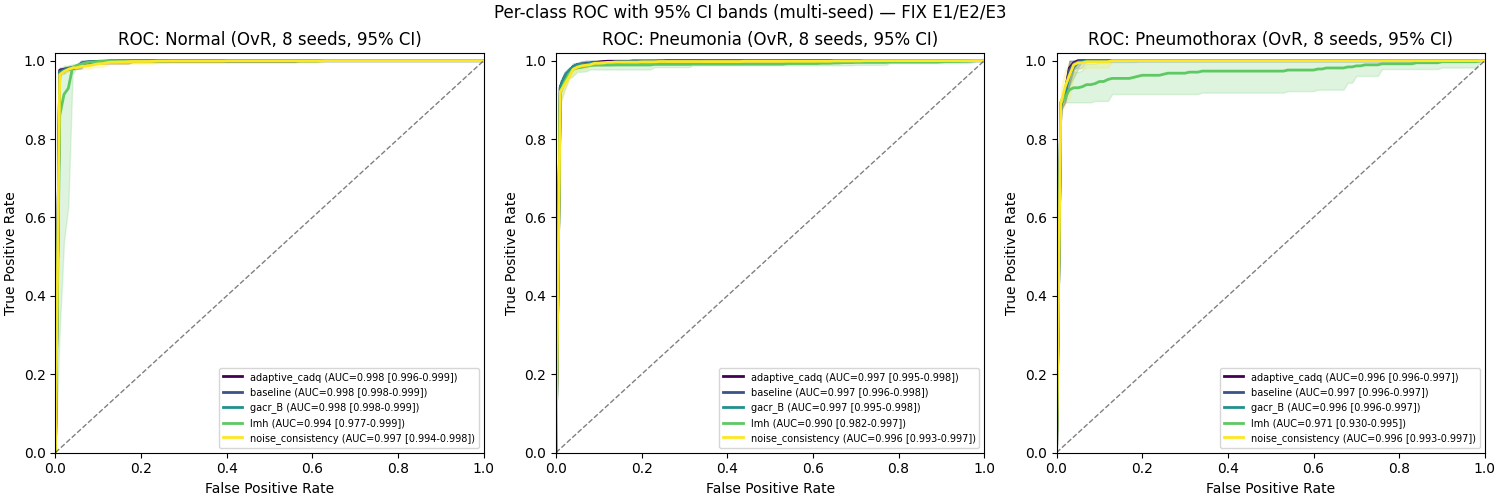
\includegraphics[width=0.82\linewidth]{roc_curves_with_ci.png}
\caption{Class-specific error and discrimination. (a) Row-normalized confusion
matrices aggregated descriptively over seeds; every row is normalized by its
true class. (b) Per-class receiver-operating-characteristic curves with
descriptive multi-seed 95\% bands. Significant DeLong results for LMH,
the noise-sensitivity (anti-consistency) condition and exploratory GACR-B reflect
lower seed-42 Pneumothorax AUROC than
baseline, not improvement. DeLong inference was not performed on subjects
pooled across seeds.}
\label{fig:error-roc}
\end{figure}

Calibration separated some conditions that had similar Macro-F1. Baseline ECE
was $0.0237\pm0.0048$ and Brier score $0.0522\pm0.0040$. LMH increased ECE
to $0.0621\pm0.0160$ (2.6-fold) and Brier score to
$0.0685\pm0.0213$; the adjusted seed-level $p$-values were 0.0313 and 0.0156.
The noise-sensitivity (anti-consistency) condition increased Brier score to
$0.0655\pm0.0130$ (adjusted $p=0.0156$), whereas its ECE change was
inconclusive. Exploratory GACR-B and
Adaptive-CADQ remained close to baseline. Figure~\ref{fig:calibration} shows
the baseline reliability diagram and seed-level ECE distributions.

\begin{figure}[pos=htbp]
\centering
\textbf{(a)}\hfill\textbf{(b)}\par\smallskip
\begin{minipage}[t]{0.43\linewidth}
\centering
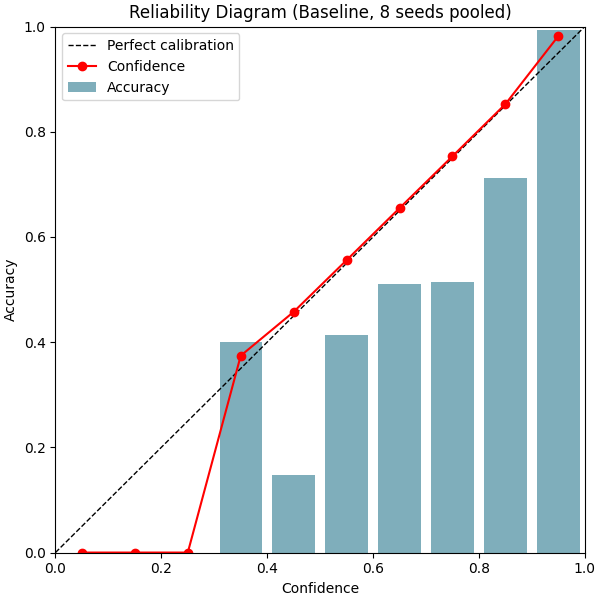
\includegraphics[width=\linewidth]{reliability_diagram.png}
\end{minipage}\hfill
\begin{minipage}[t]{0.55\linewidth}
\centering
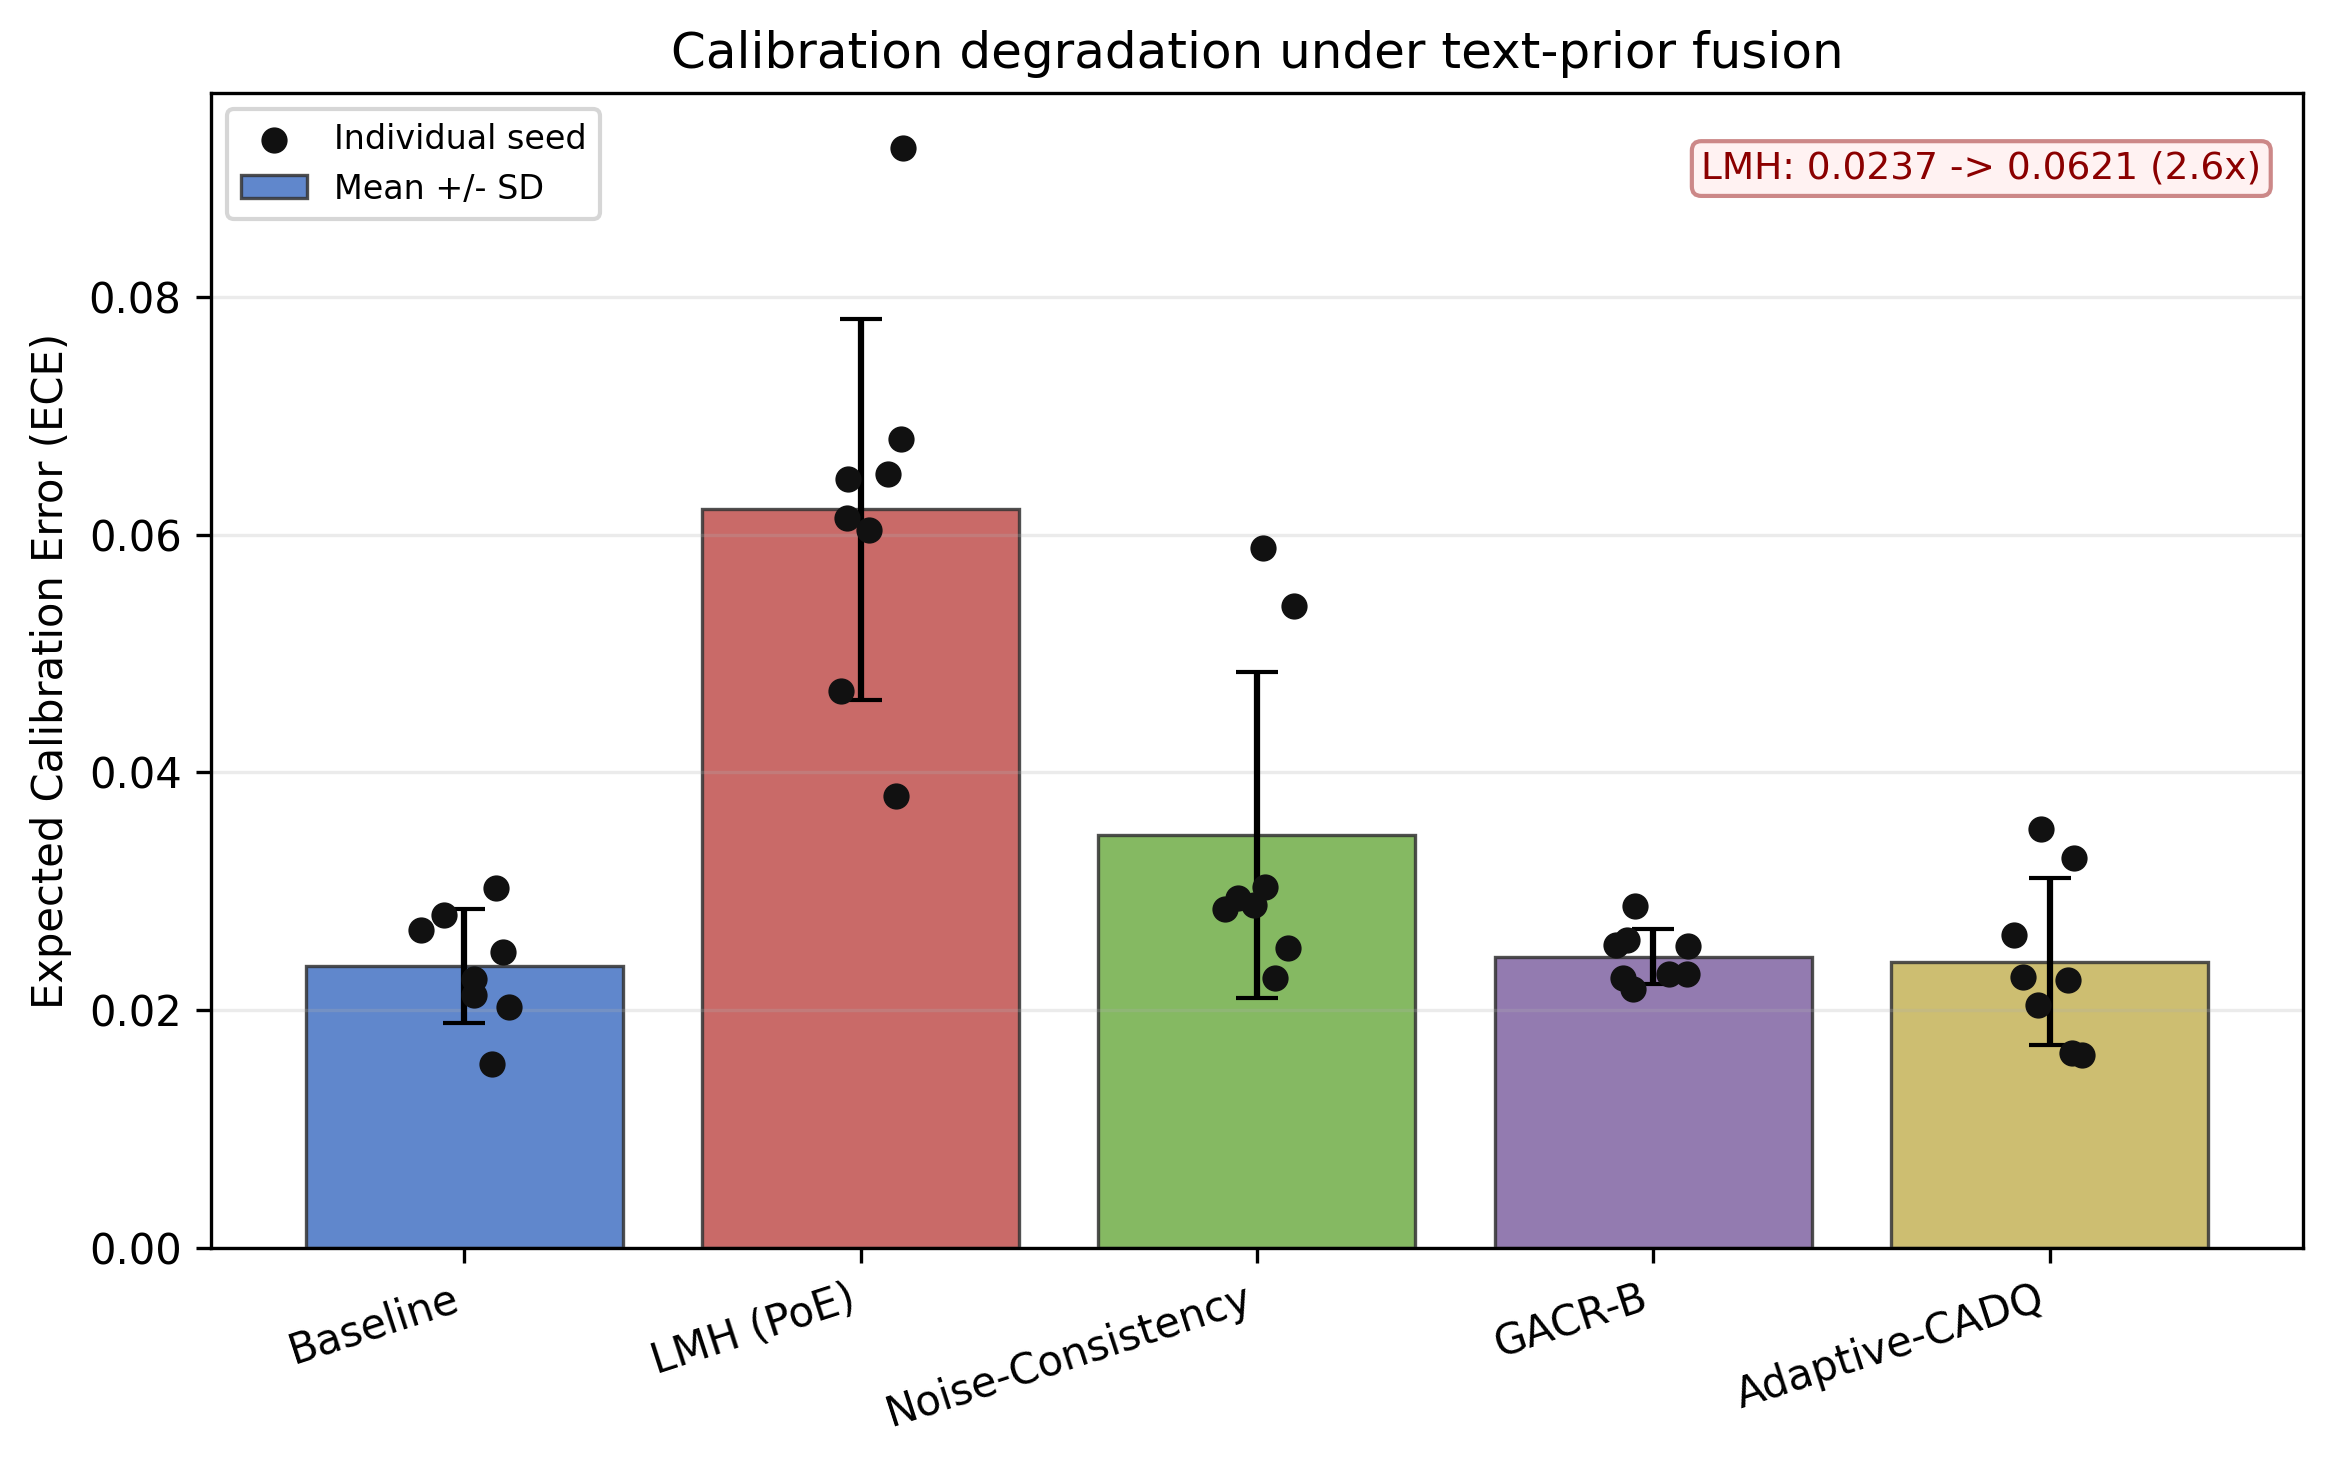
\includegraphics[width=\linewidth]{ece_seed_dots.png}
\end{minipage}
\caption{Calibration audit. (a) Descriptive baseline reliability diagram.
(b) ECE by condition with individual seed values and mean $\pm$ standard
deviation. LMH increased ECE from 0.0237 to 0.0621.}
\label{fig:calibration}
\end{figure}

\subsection{Report-preserving controls and ICM}\label{sec:icm}

The retained image-only control achieved Macro-F1 0.4611, accuracy 0.5670,
Macro-AUROC 0.6728, ECE 0.0993, and Brier score 0.6142. The text-only control
achieved 0.8555, 0.9077, 0.9820, 0.0203, and 0.1289, respectively. The
Gray-Square control achieved Macro-F1 0.9381, accuracy 0.9604, Macro-AUROC
0.9960, ECE 0.0369, and Brier score 0.0589. Its Macro-F1 was only 0.0016 below
the baseline eight-seed mean. Because these were single retained runs and the
image-only pipeline did not guarantee restoration of the best validation
checkpoint, they support an audit of
the archived system but not a definitive ranking of modality capacity.

Baseline ICM was $0.0016\pm0.0065$ with median 0.0014 and bootstrap 95\%
confidence interval $[-0.0026,0.0061]$ (Table~\ref{tab:icm}). The signed-rank
test did not reject zero ($p=0.4219$), while TOST supported equivalence inside
the operational interval ($p=0.0040$). LMH had ICM $0.0056\pm0.0098$ and did
not meet the equivalence criterion. The noise-sensitivity (anti-consistency)
condition had a negative mean ICM ($-0.0039\pm0.0081$), whereas exploratory
GACR-B and Adaptive-CADQ had small
positive values. None showed a robust positive contribution relative to the
Gray-Square reference.

\begin{table}[pos=htbp]
\centering
\caption{Image Contribution Metric statistics over eight seeds. Confidence
intervals are percentile bootstrap intervals from 2,000 resamples. Wilcoxon
tests compare ICM with zero; TOST evaluates equivalence within the operational
interval $[-0.01,0.01]$.}
\label{tab:icm}
\scriptsize
\resizebox{\linewidth}{!}{%
\begin{tabular}{lrrrrrrr}
\toprule
Condition & Mean & SD & Median & 95\% CI & Wilcoxon $p$ & TOST $p$ & Cohen's $d$ \\
\midrule
Baseline & 0.0016 & 0.0065 & 0.0014 & $[-0.0026,0.0061]$ & 0.4219 & 0.0040 & 0.247 \\
LMH (PoE) & 0.0056 & 0.0098 & 0.0066 & $[-0.0011,0.0118]$ & 0.1953 & 0.1223 & 0.566 \\
Noise-sensitivity (anti-consistency) & -0.0039 & 0.0081 & -0.0009 & $[-0.0097,0.0009]$ & 0.3828 & 0.0345 & -0.476 \\
Exploratory GACR-B & 0.0038 & 0.0062 & 0.0030 & $[-0.0002,0.0081]$ & 0.1953 & 0.0122 & 0.607 \\
Adaptive-CADQ & 0.0007 & 0.0077 & 0.0002 & $[-0.0043,0.0057]$ & 0.8438 & 0.0054 & 0.089 \\
\bottomrule
\end{tabular}}
\end{table}

The seed pairing, equivalence interval, and retained gate values are shown in
Figure~\ref{fig:icm-gates}. The Gray-Square value was reused for all eight ICM
calculations; its run-to-run uncertainty is therefore absent from the displayed
intervals. The equivalence result should be interpreted as a property of the
retained comparator, not an estimate from two independently replicated arms.

\begin{figure}[pos=htbp]
\centering
% Compact horizontal panel layout preserves the complete audit while avoiding
% an otherwise dedicated float page in the single-column review format.
\begin{minipage}[t]{0.32\linewidth}
\centering
\textbf{(a)}\par\smallskip
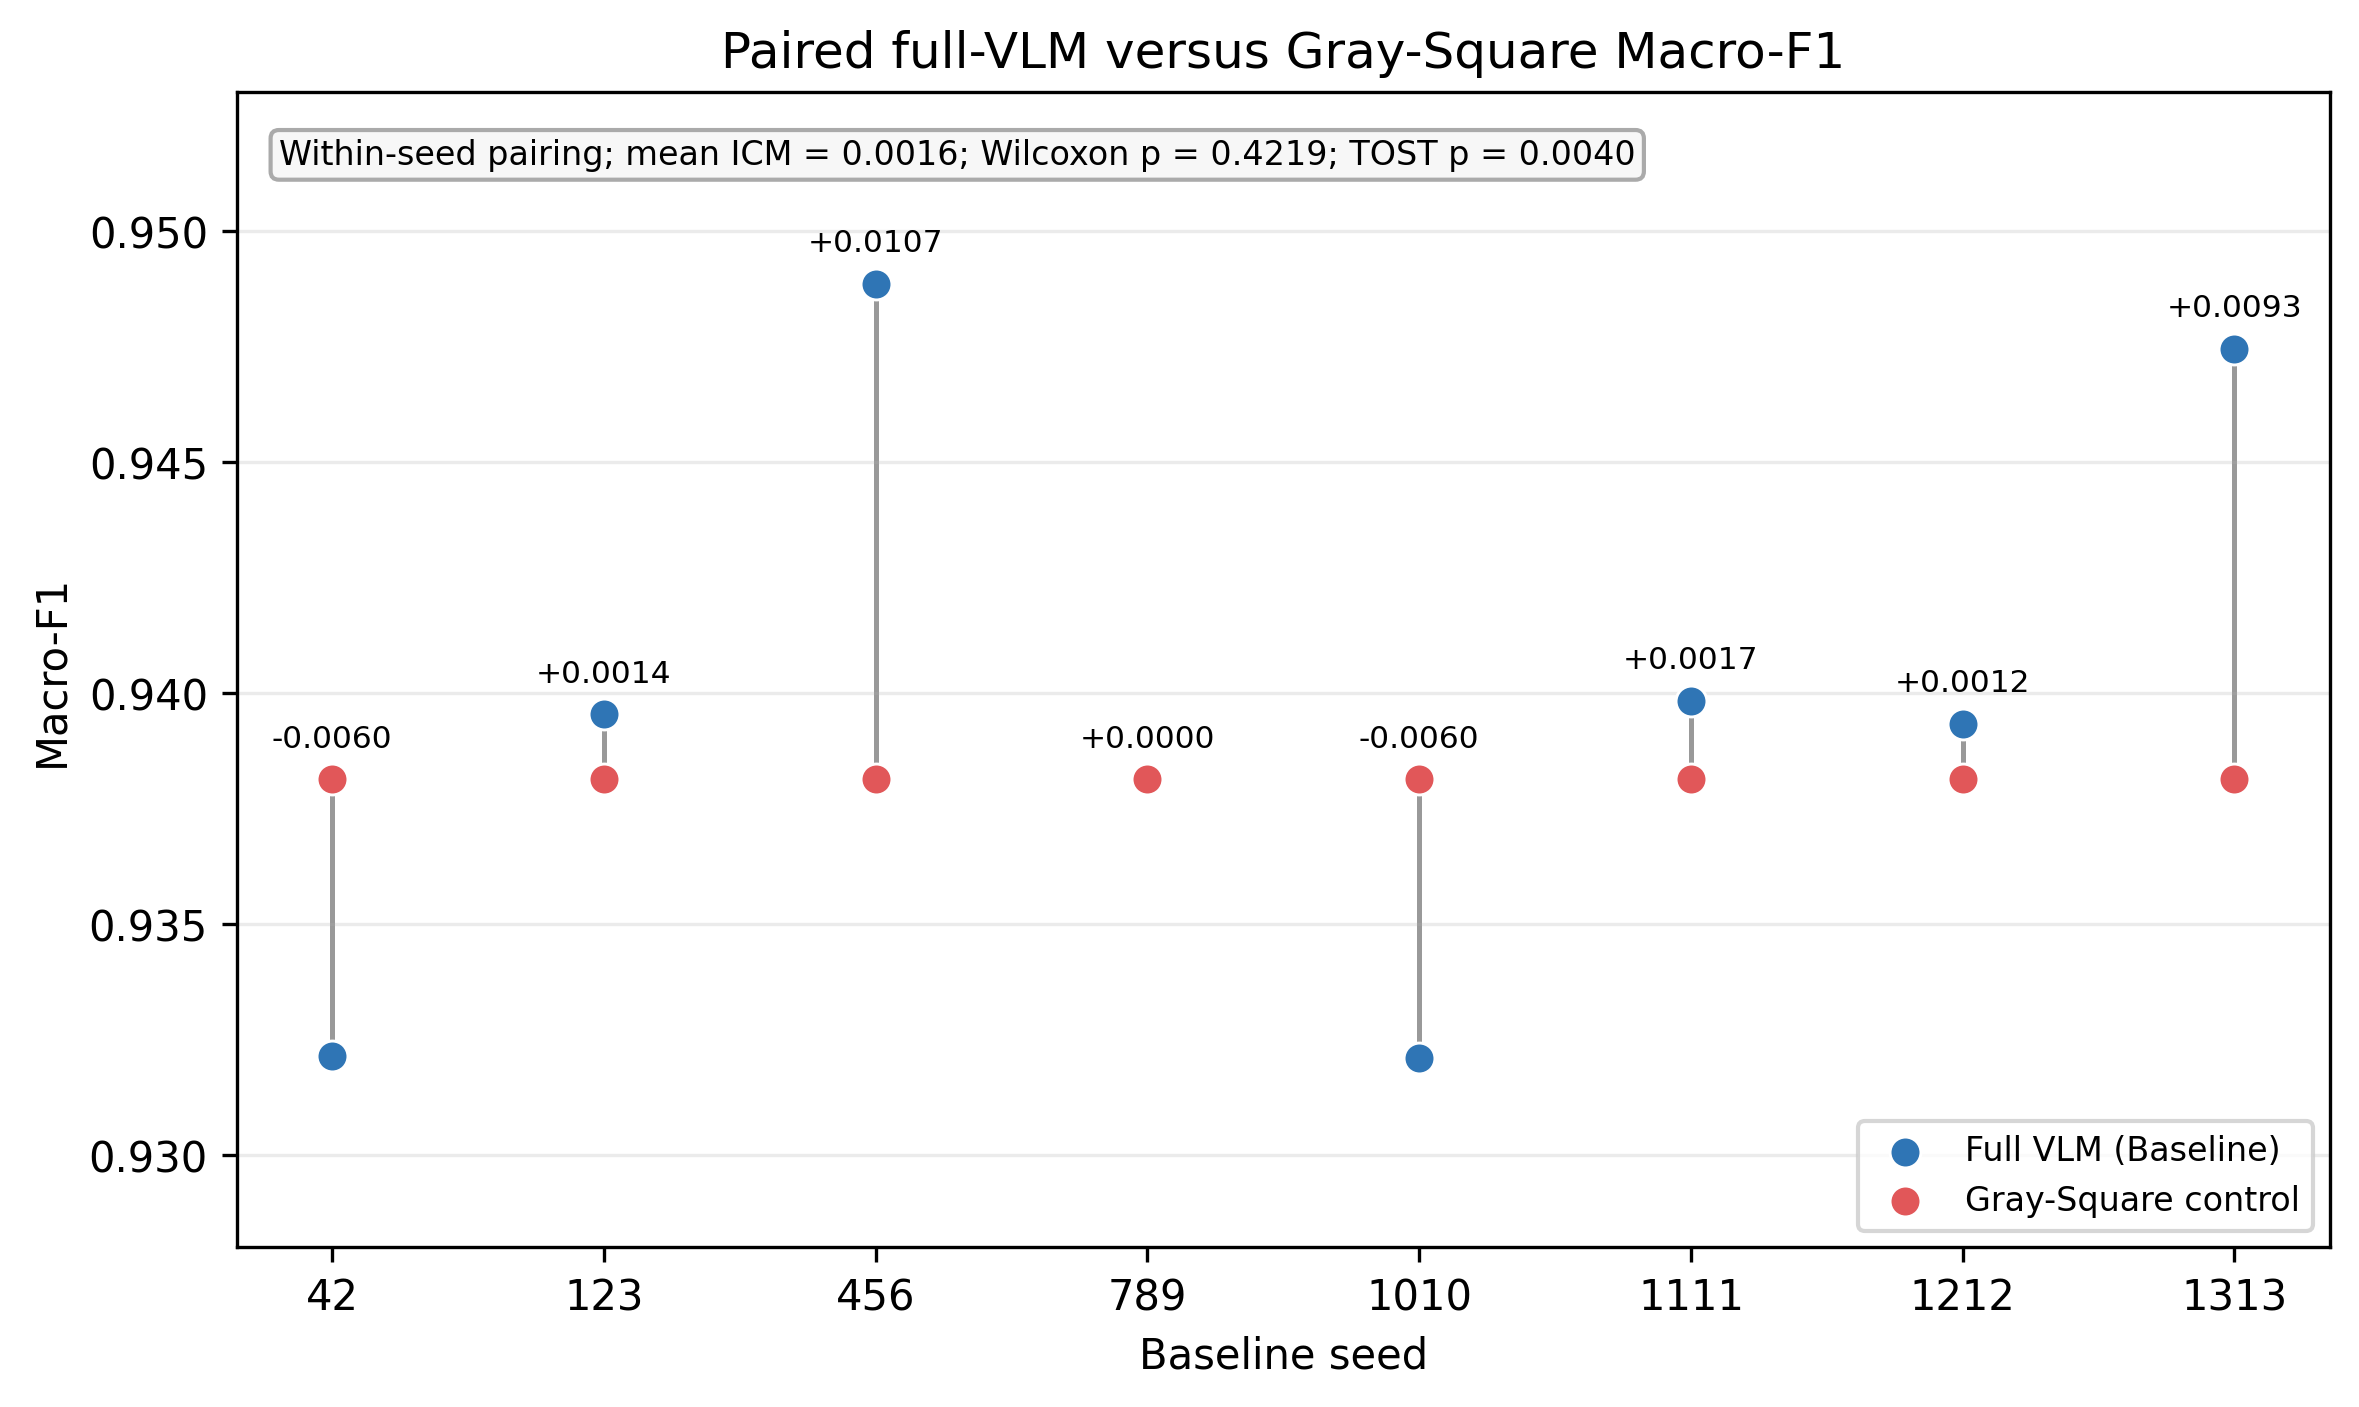
\includegraphics[width=0.98\linewidth]{paired_vlm_gray_square.png}
\end{minipage}\hfill
\begin{minipage}[t]{0.32\linewidth}
\centering
\textbf{(b)}\par\smallskip
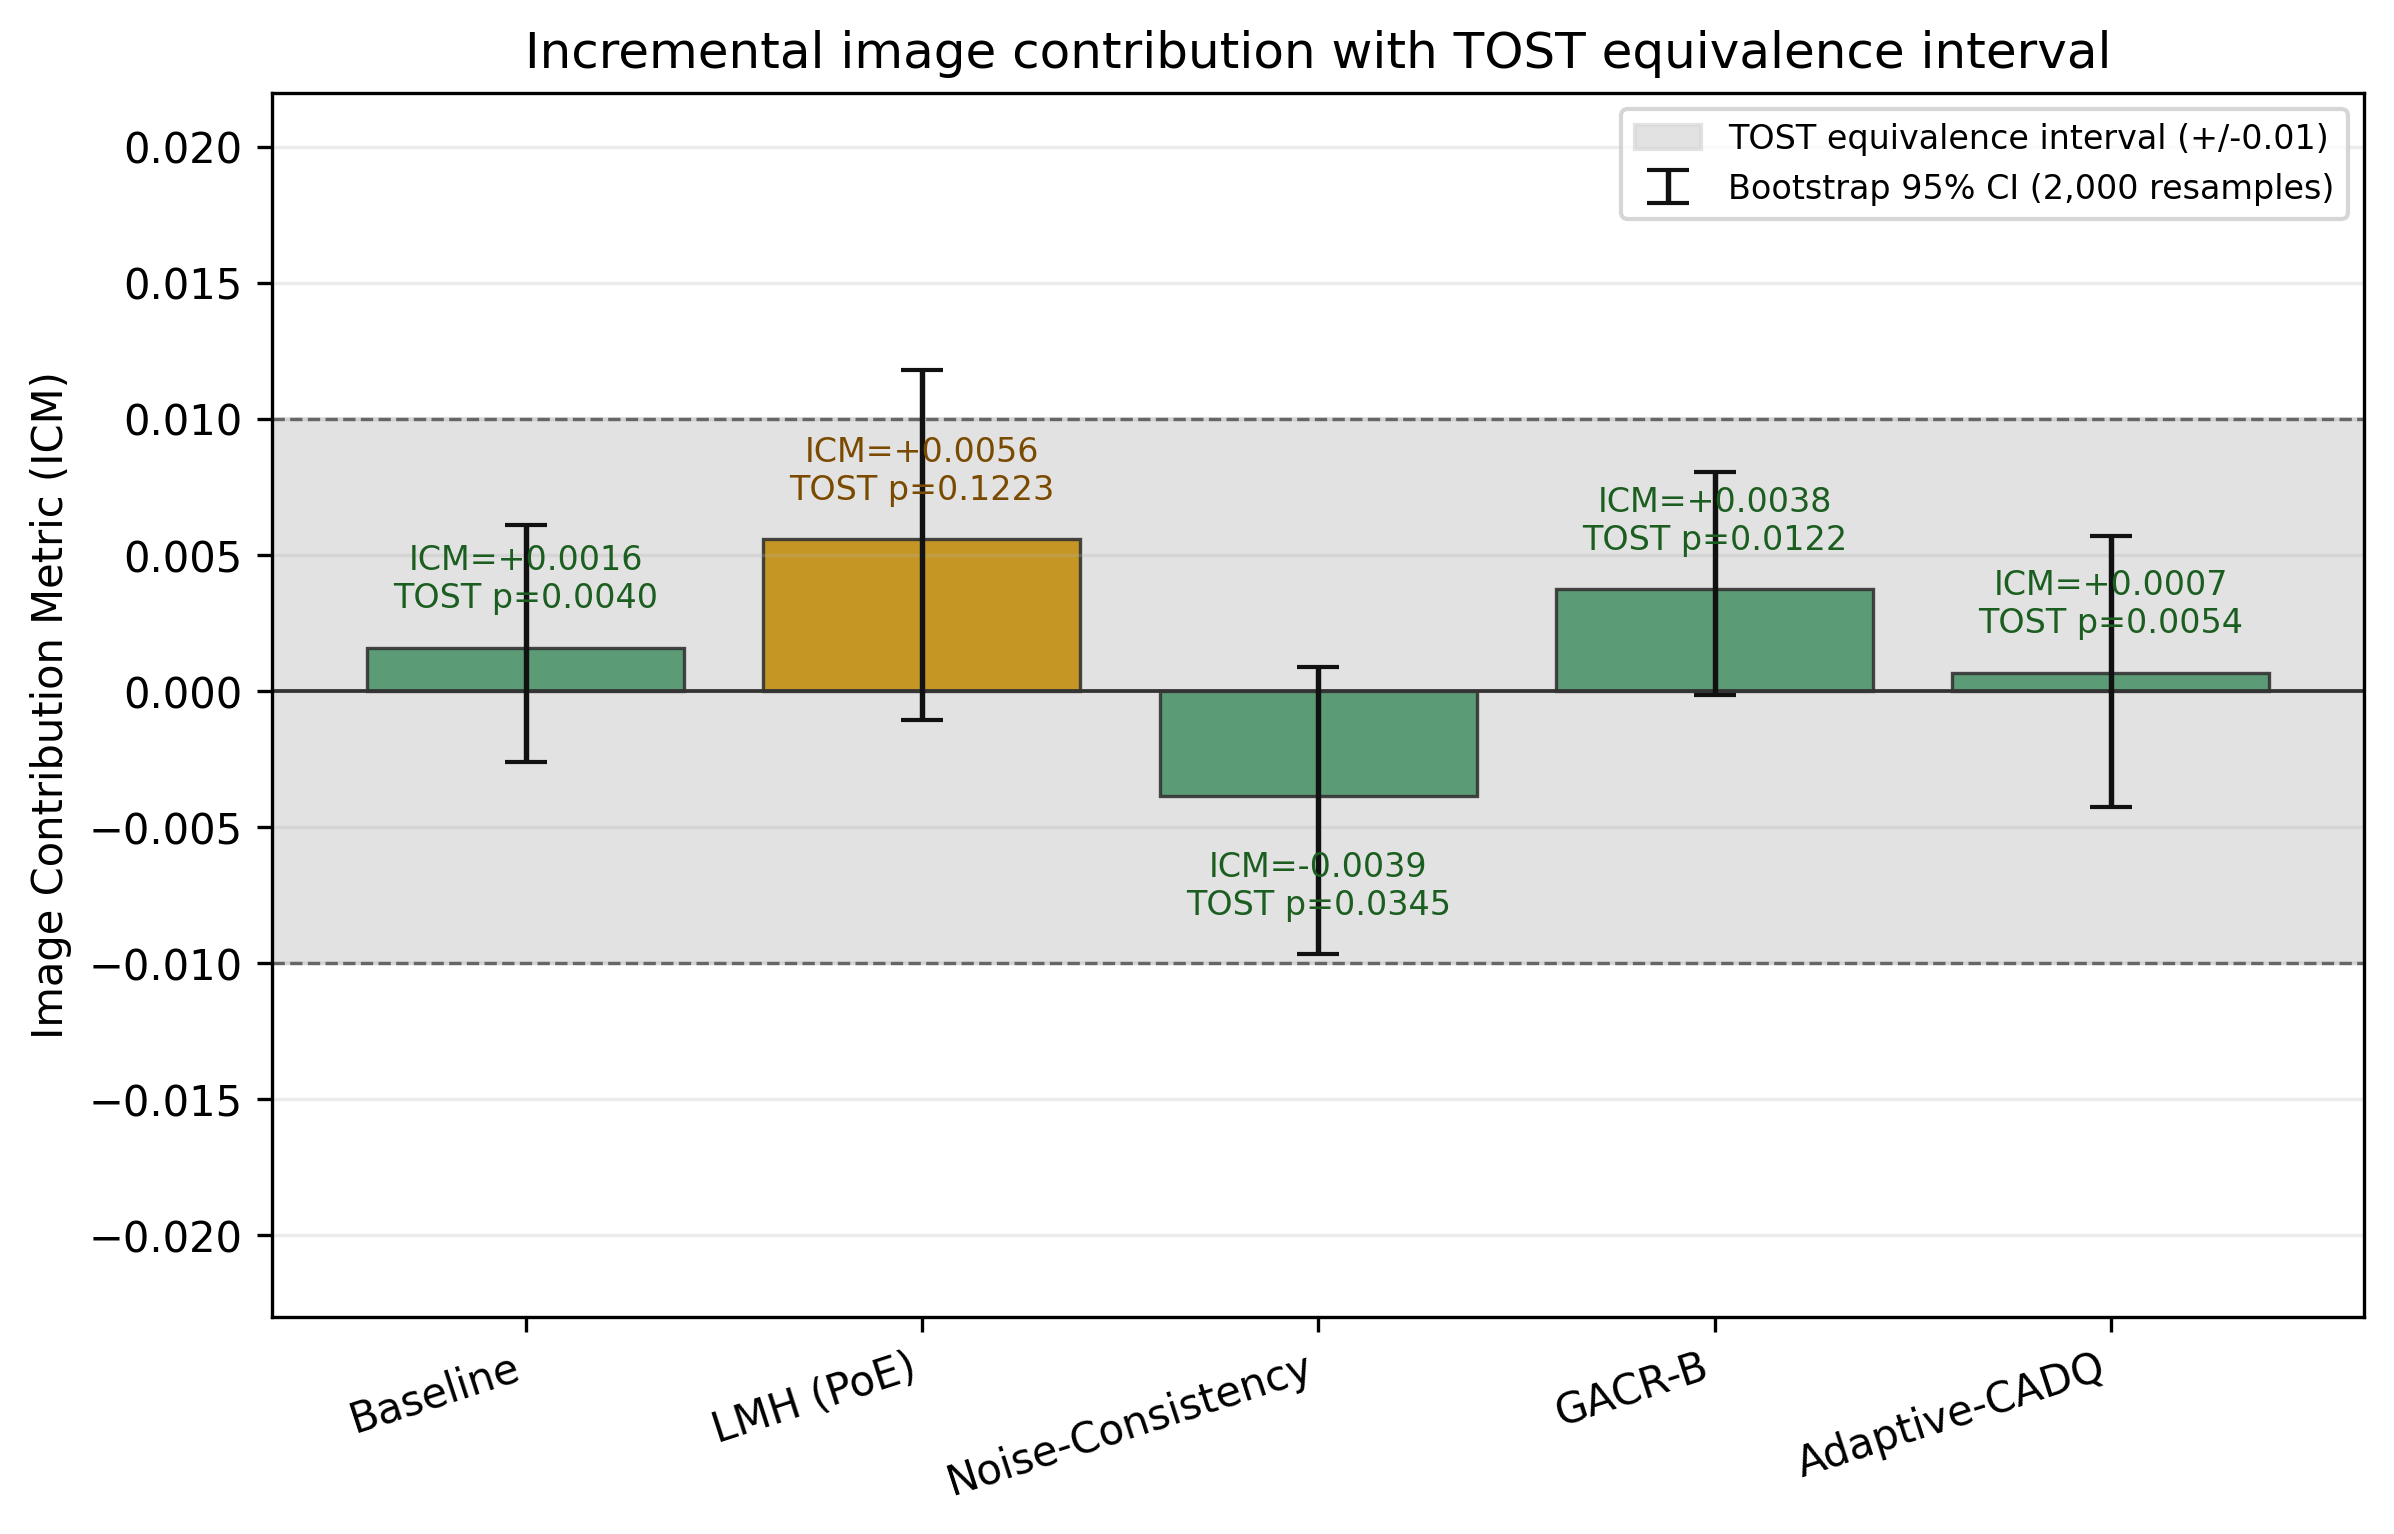
\includegraphics[width=0.98\linewidth]{icm_tost_master.png}
\end{minipage}\hfill
\begin{minipage}[t]{0.32\linewidth}
\centering
\textbf{(c)}\par\smallskip
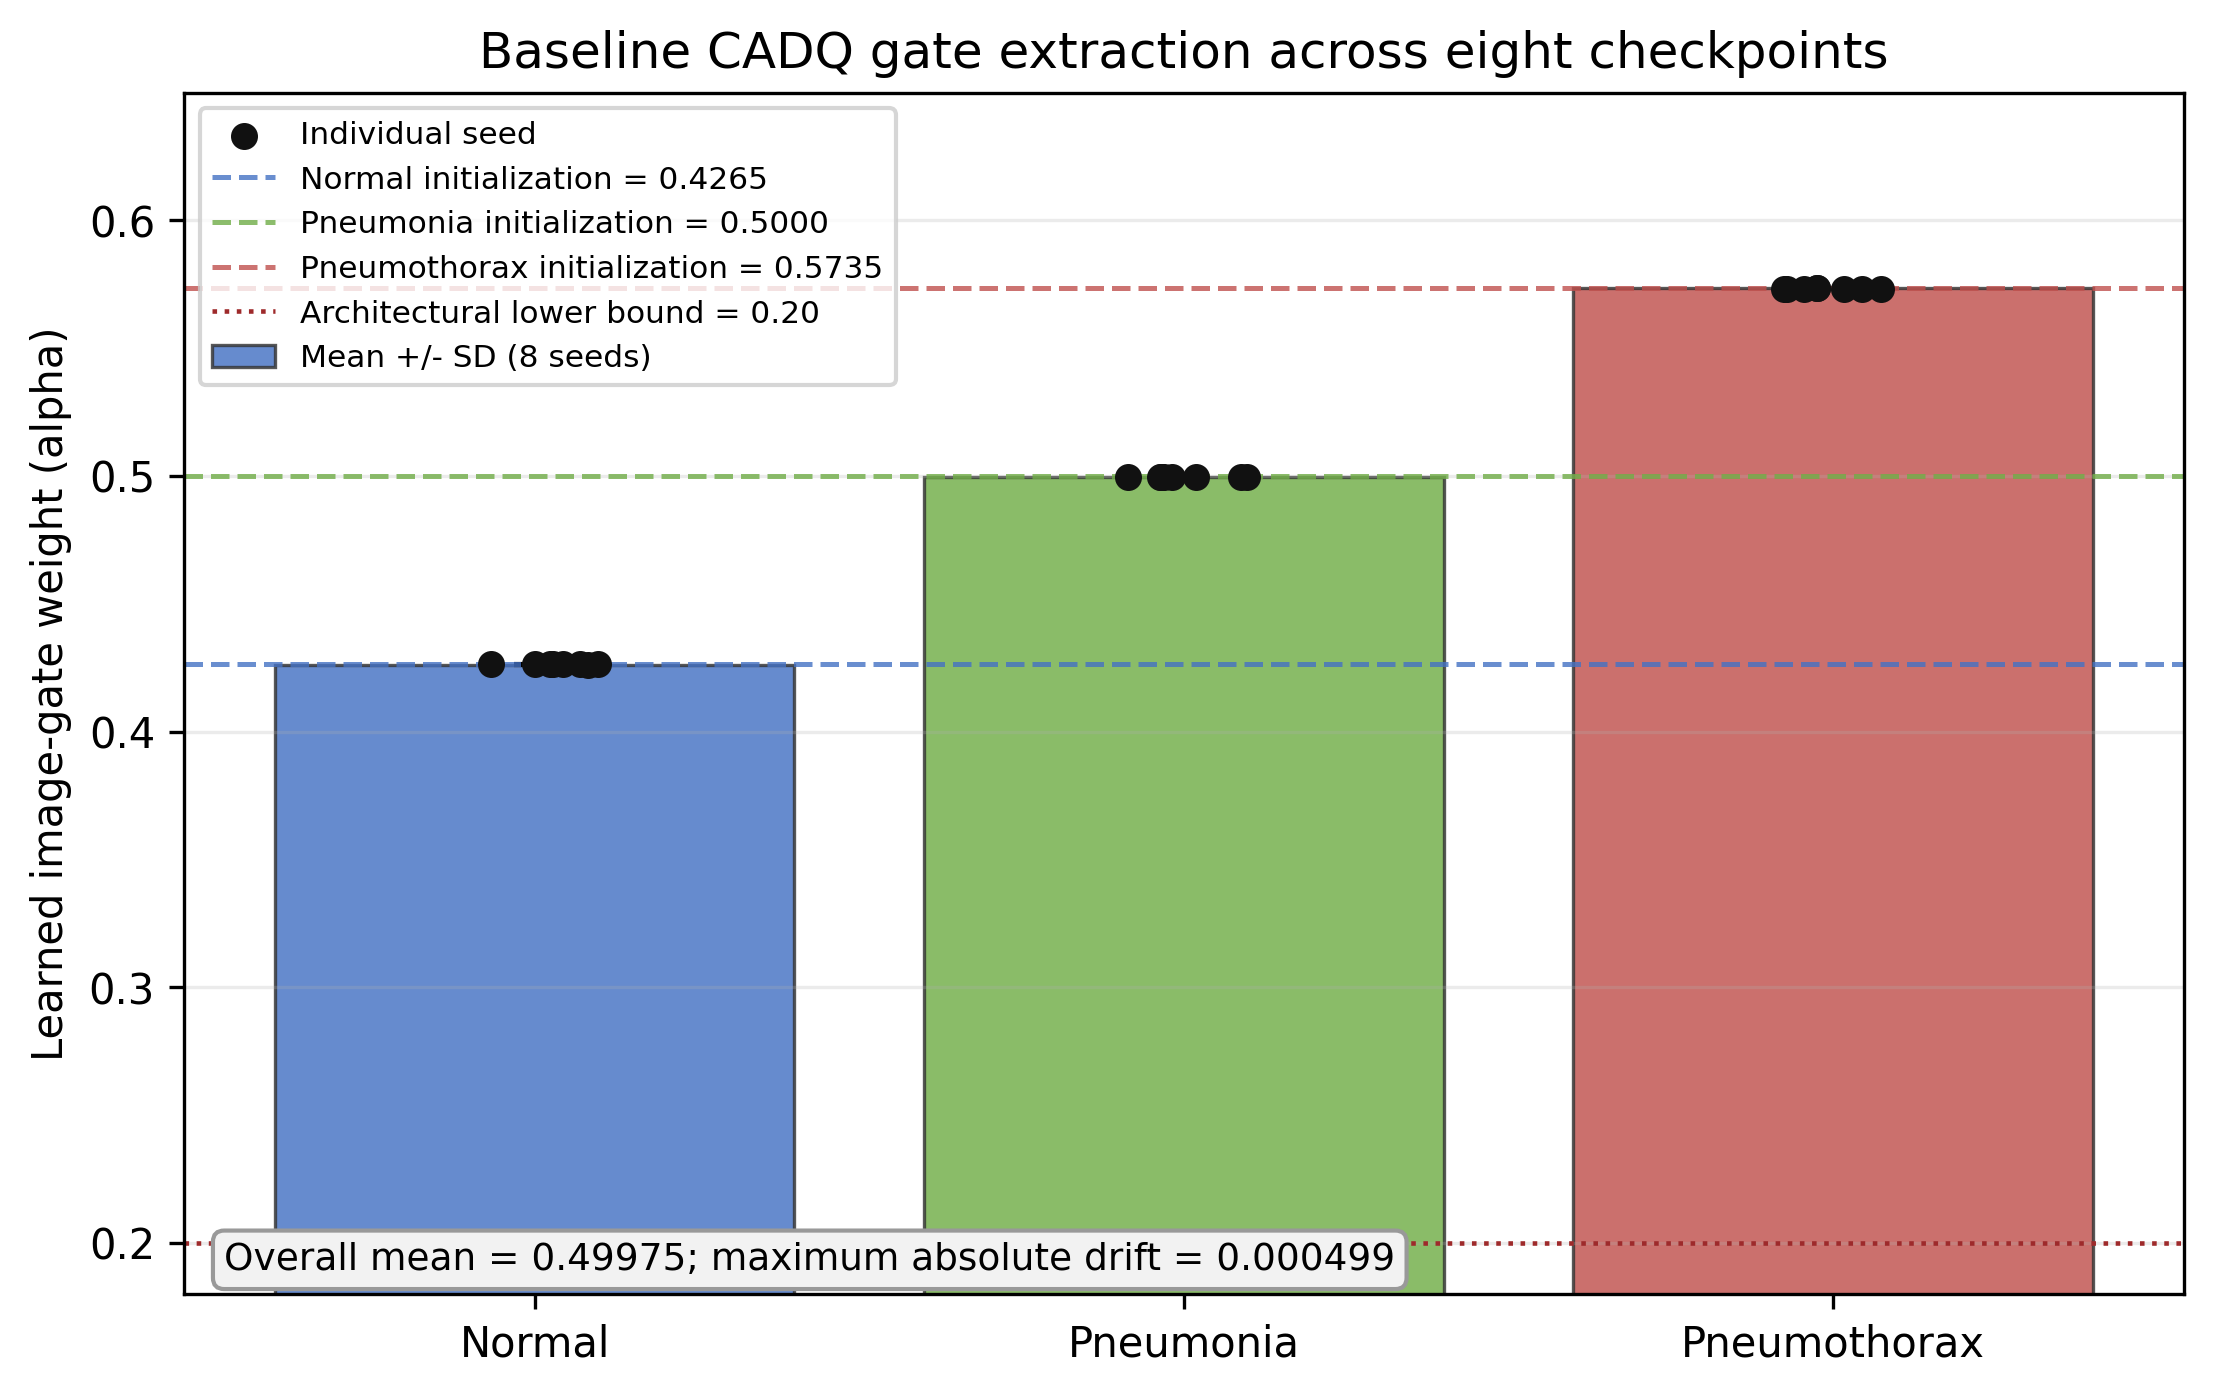
\includegraphics[width=0.98\linewidth]{gate_stagnation_with_dots.png}
\end{minipage}
\caption{Modality-contribution and gate audit. (a) Baseline VLM Macro-F1 at
each seed paired with the retained Gray-Square reference; lines show the small
differences used to construct ICM. (b) Mean ICM with percentile bootstrap 95\%
confidence intervals; shading marks the operational TOST interval
$[-0.01,0.01]$. (c) Baseline class-specific image gates from eight retained
checkpoint exports. Dots are individual seeds, bars show mean $\pm$ standard
deviation, and dashed lines are the equation-derived initial values.}
\label{fig:icm-gates}
\end{figure}

\subsection{Gate behaviour and qualitative inspection}\label{sec:gates}

The retained baseline gate means were 0.42624 for Normal, 0.49963 for
Pneumonia, and 0.57336 for Pneumothorax. The overall mean was 0.49975 compared
with an initialization mean of 0.50000, and the largest per-seed class-wise
deviation from the equation-derived initialization was 0.000499. The gate did
not collapse toward its lower bound of 0.20, nor did the retained values show a
meaningful shift toward greater image reliance. We call this descriptive pattern
\emph{gate stagnation}; it is evidence that this parameter changed little, not
proof that its gradient was exactly zero or that the image branch was
disconnected. Per-seed values appear in Supplementary Table~\ref{tab:s-gates}.

The three retained Grad-CAM examples showed diffuse activation in Baseline seed
42 (Supplementary Fig.~\ref{fig:s-gradcam}). They were not compared with
localization annotations, deletion curves, or clinician assessment. They
therefore provide only a qualitative sanity check and cannot establish visual
grounding or its absence.

% Keep the complete Results display set ahead of the interpretation.
\FloatBarrier
\section{Discussion}\label{sec:discussion}

\subsection{Principal findings and interpretation}\label{sec:principal}

The central result is a mismatch between high predictive performance and
incremental image evidence. Baseline Macro-F1 approached 0.94, yet a constant
gray image paired with the same report retained Macro-F1 0.9381. Baseline ICM
was close to zero, its signed-rank test was non-significant, and TOST supported
equivalence within the project-defined interval. None of the four alternative
fusion or text-debiasing conditions produced a robust ICM increase. The LMH
text-prior intervention had the highest mean Macro-F1 but lower AUROC and much
worse calibration. The retained baseline gates stayed close to initialization.
Together, these findings show that aggregate performance, a non-collapsed gate,
and visually plausible activation maps can coexist with negligible performance
change after image replacement.

The most direct explanation is construct overlap. MIMIC-CXR pairs each image
with a report, CheXpert uses report language to generate the target, and the
model receives the report's \texttt{findings} field
\cite{johnson2019mimiccxr,irvin2019chexpert}. The Gray-Square control preserves
this high-information route. It does not show that the CheXpert labels are
clinically inaccurate, that every prediction copied a particular phrase, or that
radiographs lack diagnostic value. It shows that the evaluated endpoint does
not isolate independent image-based recognition. The claim supported by the
data is therefore narrow: under this report-linked setup and archived
implementation, the measured incremental image contribution was negligible.

We use \emph{modality inertia} to describe the combined observation that the
output changes little under report-preserving image replacement while the
static gate remains near its starting value. This is a useful diagnostic label,
but the current experiment does not identify a unique mechanism. Redundant
features, optimization dynamics, precision, normalization mismatch, or weak
image gradients could each contribute. The gate result should not be promoted
from a parameter-stability observation to proof of causal gradient starvation
without gradient traces or controlled retraining.

The debiasing results clarify why endpoint design matters. Product-of-experts
methods are intended to suppress an easy language prior. Here, however, report
language helped generate the target. Down-weighting this pathway can degrade
AUROC or calibration without creating new image information, as observed for
LMH. The noise-sensitivity (anti-consistency) condition cannot support its
intended conventional-consistency interpretation because its archived
negative-KL formulation rewards divergence. Adaptive-CADQ changed the gate form
but not the endpoint. Exploratory GACR-B, following the grounding-aware
proposal of Sadanandan and Behzadan
\cite{sadanandan2026consistentdangerous}, achieved a small ICM but not a robust
Macro-F1 improvement. The experiment did not measure whether its $\lambda=0.3$
penalty generated insufficient gradient; that mechanism requires a dedicated
ablation and is not inferred from the null performance result.

The corrected McNemar interpretation is also important. Exploratory GACR-B and
Adaptive-CADQ had $p=1.000$, but both had non-zero discordant predictions. The
off-diagonal counts were nearly balanced, so McNemar detected no directional
change in error rates. This supports a conclusion of similar aggregate paired
behaviour, not byte-identical decision boundaries. Reporting the contingency
counts prevents a non-significant symmetry test from being mistaken for an
identity test.

\subsection{Implications for biomedical informatics}\label{sec:implications}

Multimodal evaluation should make modality contribution explicit. A minimum
audit should document how targets were produced, whether any input shares that
source, what happens when each modality is replaced or permuted, whether
controls are matched across seeds, and how calibration changes. The ablation
must preserve all other inputs and the evaluation cohort. Where the scientific
claim is that an image contributes, an independent or image-derived reference
standard is preferable to a target extracted from the accompanying report.
Counterfactual text tests, temporally separated note fields, and cross-patient
report swaps can further reveal which source carries the prediction.

ICM is one compact summary of such an intervention. Its advantages are an
interpretable direction and a model-relative scale, but it inherits every
limitation of the chosen performance metric and comparator. Macro-F1 may hide
class-specific harm; a single Gray-Square run understates control uncertainty;
and the $[-0.01,0.01]$ interval has not been clinically validated. ICM should
therefore be reported with absolute performance, per-class outcomes,
calibration, confidence intervals, and a description of the control. Validation
on independent-label tasks is needed before comparing ICM across datasets.

Gate and saliency analyses should remain secondary. A gate is shaped by
parameterization and can be unidentifiable when modality signals are redundant.
The one-key attention block used here cannot align words to image regions, and
three Grad-CAM examples lack quantitative localization evidence. A stronger
future design would use token- and region-level interactions, paired modality
interventions, gradient and gate trajectories, concept localization, and
reader-validated explanations. Even then, behavioural change under input
intervention remains the more direct evidence of contribution.

For regulatory-facing evidence, the central lesson is traceability rather than
a proposed mandatory threshold. Good machine-learning-practice and real-world-
evidence principles emphasize representative evaluation, transparent data
provenance, uncertainty, and evidence aligned with intended use
\cite{fda2025gmlp,fda2025rwe}. A multimodal device dossier should therefore
state whether labels and inputs share provenance and include matched ablations
when modality use is part of the intended claim. ICM and gate inspection can
support that evidence package, but neither substitutes for external validation,
clinical utility, subgroup performance, or human-factors assessment.

\subsection{Limitations and future work}\label{sec:limitations}

This audit has substantial limitations. It used 2,953 studies from one
database, one labeler, three classes, and only 47 Pneumothorax test studies. The
uncertain-to-negative mapping, class caps, prevalence, and inherited split may
affect the results. No external cohort, radiologist-adjudicated reference,
prospective workflow, reader study, subgroup analysis, decision-curve analysis,
or outcome evaluation was available. Generalization to other reports,
institutions, devices, and label processes is unknown.

Implementation limitations constrain causal interpretation. Image values were
mapped to $[-1,1]$, which may not match the native TorchXRayVision convention
for the selected weights. The noise-sensitivity (anti-consistency) condition
used a negative-KL formulation that rewards divergence. The attention block
used one token per modality. Image-only checkpoint restoration did not
guarantee the best validation checkpoint, so that control is descriptive.
The affected conditions are interpreted as probes of the archived system's
behaviour under a report-linked endpoint. ICM and condition contrasts are the
primary evidence within this setting; shared preprocessing does not establish
that those comparisons are unaffected by its limitations.

Control and statistical asymmetries also matter. The same single Gray-Square
run was reused to construct eight ICM values, so comparator uncertainty was not
propagated. Eight seeds provide a small replication sample. DeLong and McNemar
results were computed only from the retained seed-42 arrays, whereas
seed-aggregated curves are descriptive. Adaptive-CADQ's eight-seed extension and
exploratory GACR-B were post hoc. No a priori sample-size calculation established power for
a clinically meaningful ICM. Future studies should train every control at every
seed, preregister the equivalence margin and estimand, and use a larger
independent-label cohort.

Finally, the result archive was assembled from multiple notebook outputs. The
merge retained first-seen duplicates without a documented source-priority rule
or content hashes, and some probabilities had to be recovered from a companion
pickle. A confirmatory release should include a locked environment, dataset and
split hashes, notebook and checkpoint hashes, deterministic merge rules, full
probability arrays, and a machine-readable provenance manifest. The present
manifest is descriptive and identifies rather than resolves these issues.

\section{Conclusion}\label{sec:conclusion}

In this MIMIC-CXR-derived task, replacing the radiograph with a constant image
preserved nearly all baseline Macro-F1. Baseline ICM was near zero and equivalent
within the operational interval, the tested interventions did not demonstrate a
robust increase in incremental image contribution, and retained static gates
remained near initialization. These findings expose a benchmark-validity risk
created when labels and text inputs share report provenance. They do not show
that radiographs or medical VLMs are generally uninformative. Independent
labels, implementation validation, matched multi-seed controls, provenance
locking, and external validation are required. ICM is best used as one component
of a broader modality-reliance audit.

\section*{Ethics approval and consent to participate}
MIMIC-CXR is de-identified and was accessed through official PhysioNet
credentialing under its Data Use Agreement. No participants were recruited, no
direct identifiers were accessed, and consent was not applicable. The source
resource was released under the originating institutional review-board
approvals; this secondary computational analysis introduced no intervention or
participant contact.

\section*{Data availability}
Raw MIMIC-CXR images and reports remain under PhysioNet access controls and are
not redistributed. Non-identifying summaries, code, manuscript source, and
figure-generation materials are available at
\url{https://github.com/i-mTanvir/MediVision}. Cohort identifiers can be shared
only in a manner consistent with the PhysioNet Data Use Agreement.

\section*{Code availability}
The analysis notebooks, LaTeX source, figure scripts, and environment records
are available at \url{https://github.com/i-mTanvir/MediVision}. A permanent
archival DOI will be added if a versioned release is deposited. Credentials,
raw reports, and restricted identifiers are excluded.

\section*{Funding}
This research received no specific grant from public, commercial, or
not-for-profit funding bodies and was self-funded by the authors. No external
sponsor influenced the design, analysis, interpretation, writing, or decision
to submit.

\section*{Declaration of competing interest}
The authors declare no known competing financial interests or personal
relationships that could have influenced this work.

\section*{Author contributions}
Nafis Al Rahman and Tanvir Mahmud contributed equally to conceptualization,
methodology, investigation, software, data curation, formal analysis,
validation, visualization, and writing. Both authors reviewed and approved the
manuscript and accept responsibility for its content.

\section*{Acknowledgements}
The authors thank PhysioNet and the MIMIC-CXR data custodians for maintaining
the de-identified resource and controlled-access infrastructure.

\section*{Declaration of generative AI and AI-assisted technologies in the writing process}
Generative-AI tools were not used to generate study data, execute experiments,
create scientific results, or make analytical decisions. Any language or
formatting assistance used during manuscript preparation was reviewed and
edited by both authors, who take full responsibility for the final content.

\clearpage
\appendix
\setcounter{table}{0}
\setcounter{figure}{0}
\renewcommand{\thesection}{S}
\renewcommand{\thetable}{S\arabic{table}}
\renewcommand{\thefigure}{S\arabic{figure}}
\section{Supplementary material}

\subsection{Per-seed gate values}

\begin{table}[pos=H]
\centering
\caption{Baseline CADQ image-gate values retained in the checkpoint export.
Initialization values are $(0.426524,0.500000,0.573476)$. Maximum drift is the
largest absolute class-wise difference from initialization for that seed.}
\label{tab:s-gates}
\scriptsize
\begin{tabular}{r rrr r}
\toprule
Seed & Normal $\alpha$ & Pneumonia $\alpha$ & Pneumothorax $\alpha$ & Max drift \\
\midrule
42   & 0.426270 & 0.499512 & 0.573242 & 0.000488 \\
123  & 0.426270 & 0.499512 & 0.573730 & 0.000488 \\
456  & 0.426025 & 0.499756 & 0.573242 & 0.000499 \\
789  & 0.426270 & 0.499756 & 0.573242 & 0.000255 \\
1010 & 0.426270 & 0.499756 & 0.573242 & 0.000255 \\
1111 & 0.426270 & 0.499512 & 0.573242 & 0.000488 \\
1212 & 0.426270 & 0.499756 & 0.573730 & 0.000255 \\
1313 & 0.426270 & 0.499512 & 0.573242 & 0.000488 \\
\bottomrule
\end{tabular}
\end{table}

\subsection{Training configuration}

\begin{table}[pos=H]
\centering
\caption{Training hyperparameters for the archived experiments.}
\label{tab:s-hyperparameters}
\scriptsize
\begin{tabular}{p{0.31\linewidth}p{0.61\linewidth}}
\toprule
Setting & Value \\
\midrule
Image encoder & TorchXRayVision DenseNet-121, res224 MIMIC weights \\
Text encoder & Bio\_ClinicalBERT; first four transformer layers frozen \\
Optimizer & AdamW; weight decay $10^{-4}$ \\
Learning rates & $10^{-5}$ image/text; $10^{-4}$ heads; $5\times10^{-5}$ static gates \\
Schedule & OneCycleLR with 10\% warm-up; 10 epochs \\
Batching & Physical batch 8; four accumulation steps; effective batch 32 \\
Objective & Focal cross-entropy ($\gamma=1.5$), label smoothing 0.05, effective-number $\beta=0.99$ \\
Precision & FP16 mixed precision with gradient scaling \\
Gate initialization & $u=(-0.5,0,0.5)$; $\alpha=(0.426524,0.500000,0.573476)$ \\
Augmentation & Crop, flip, rotation, translation, intensity jitter; minority-class transform \\
Seeds & 42, 123, 456, 789, 1010, 1111, 1212, 1313 \\
Hardware & Kaggle NVIDIA T4 two-GPU environment \\
\bottomrule
\end{tabular}
\end{table}

\subsection{Reporting-checklist summaries}

\begin{table}[pos=H]
\centering
\caption{CLAIM 2024 audit summary. Counts reproduce the archived 27-item
project audit; full item-level responses remain in the repository.}
\label{tab:s-claim}
\scriptsize
\begin{tabular}{lcp{0.66\linewidth}}
\toprule
Status & Count & Summary \\
\midrule
Yes & 13 & Study type, source, outcome, model description, metrics, comparisons, limitations, and seed-level analysis were reported. \\
Partial & 10 & External validation, comparator breadth, ablation coverage, and reproducibility were limited by scope and controlled data access. \\
No & 4 & Cross-validation, external state-of-the-art baselines, pretraining-overlap audit, and complete credentialing documentation were not included. \\
\bottomrule
\end{tabular}
\end{table}

\begin{table}[pos=H]
\centering
\caption{TRIPOD+AI audit summary. Counts reproduce the archived 41-item project
audit; full item-level responses remain in the repository.}
\label{tab:s-tripod}
\scriptsize
\begin{tabular}{lcp{0.66\linewidth}}
\toprule
Status & Count & Summary \\
\midrule
Yes & 9 & The title, data source, participants, model, statistical tests, limitations, registration history, and availability statements were addressed. \\
Partial & 18 & Abstract detail, hyperparameters, comparison breadth, reproducibility, and ethics reporting were only partly addressed. \\
No & 14 & External validation, decision-curve analysis, subgroup/fairness analysis, missing-data assessment, calibration transfer, and a model card were absent. \\
\bottomrule
\end{tabular}
\end{table}

\subsection{Provenance manifest}

\begin{table}[pos=H]
\centering
\caption{Condition-level provenance and known constraints in the fixed archive.}
\label{tab:s-provenance}
\scriptsize
\begin{tabular}{p{0.18\linewidth}p{0.18\linewidth}p{0.22\linewidth}p{0.32\linewidth}}
\toprule
Condition & Seed coverage & Retained outputs & Known constraint \\
\midrule
Baseline CADQ & 8 seeds & Metrics, predictions, probabilities, gates & Image normalization requires confirmation against XRV convention \\
LMH (PoE) & 8 seeds & Metrics, predictions, probabilities & Warm-started; calibration degraded \\
Noise-sensitivity (anti-consistency) & 8 seeds & Metrics, predictions, probabilities & Negative-KL formulation rewards divergence \\
Exploratory GACR-B & 8 seeds & Metrics, predictions, recovered probabilities & Added post hoc; merge provenance was not hash-locked \\
Adaptive-CADQ & 8 seeds & Metrics, predictions, probabilities & Extended from three to eight seeds post hoc \\
Controls & One retained run each & Metrics and selected arrays & Gray-Square uncertainty not replicated; image-only best-checkpoint restoration was not uniform \\
\bottomrule
\end{tabular}
\end{table}

\subsection{Seed-42 sensitivity intervals}

\begin{table}[pos=H]
\centering
\caption{Seed-42 per-class sensitivity with Wilson 95\% confidence intervals
($n=455$; Normal $n=240$, Pneumonia $n=168$, Pneumothorax $n=47$).}
\label{tab:s-wilson}
\scriptsize
\begin{tabular}{lccc}
\toprule
Condition & Normal & Pneumonia & Pneumothorax \\
\midrule
Baseline & 0.975 [0.946, 0.988] & 0.947 [0.903, 0.972] & 0.894 [0.774, 0.954] \\
LMH (PoE) & 0.962 [0.929, 0.980] & 0.947 [0.903, 0.972] & 0.894 [0.774, 0.954] \\
Noise-sensitivity (anti-consistency) & 0.962 [0.929, 0.980] & 0.947 [0.903, 0.972] & 0.894 [0.774, 0.954] \\
Exploratory GACR-B & 0.975 [0.946, 0.988] & 0.947 [0.903, 0.972] & 0.894 [0.774, 0.954] \\
Adaptive-CADQ & 0.979 [0.952, 0.991] & 0.953 [0.910, 0.976] & 0.894 [0.774, 0.954] \\
\bottomrule
\end{tabular}
\end{table}

\subsection{Qualitative saliency examples}

\begin{figure}[pos=H]
\centering

\includegraphics[width=0.72\linewidth]{gradcam_baseline.png}
\caption{Qualitative Grad-CAM examples for Baseline seed 42. The examples were
not evaluated against localization annotations and do not support a causal or
quantitative grounding claim.}
\label{fig:s-gradcam}
\end{figure}

% JBI uses numbered references in first-citation order.
\bibliographystyle{elsarticle-num}
\renewcommand{\bibfont}{\fontsize{7pt}{8pt}\selectfont}
\begingroup
\sloppy
% Keep long web addresses from overflowing the single-column reference list.
\renewcommand{\url}[1]{\href{#1}{\texttt{link}}}
\bibliography{related_work_references,methodology_references}
\endgroup

\end{document}
